% ----------------------------------------------------------------------
%
%                            TFMTesis.tex
%
%----------------------------------------------------------------------
%
% Este fichero contiene el "documento maestro" del documento. Lo único
% que hace es configurar el entorno LaTeX e incluir los ficheros .tex
% que contienen cada sección.
%
%----------------------------------------------------------------------
%
% Los ficheros necesarios para este documento son:
%
%       TeXiS/* : ficheros de la plantilla TeXiS.
%       Cascaras/* : ficheros con las partes del documento que no
%          son capítulos ni apéndices (portada, agradecimientos, etc.)
%       Capitulos/*.tex : capítulos de la tesis
%       Apendices/*.tex: apéndices de la tesis
%       constantes.tex: constantes LaTeX
%       config.tex : configuración de la "compilación" del documento
%       guionado.tex : palabras con guiones
%
% Para la bibliografía, además, se necesitan:
%
%       *.bib : ficheros con la información de las referencias
%
% ---------------------------------------------------------------------

\documentclass[12pt,a4paper,twoside]{book}

%
% Definimos  el   comando  \compilaCapitulo,  que   luego  se  utiliza
% (opcionalmente) en config.tex. Quedaría  mejor si también se definiera
% en  ese fichero,  pero por  el modo  en el  que funciona  eso  no es
% posible. Puedes consultar la documentación de ese fichero para tener
% más  información. Definimos también  \compilaApendice, que  tiene el
% mismo  cometido, pero  que se  utiliza para  compilar  únicamente un
% apéndice.
%
%
% Si  queremos   compilar  solo   una  parte  del   documento  podemos
% especificar mediante  \includeonly{...} qué ficheros  son los únicos
% que queremos  que se incluyan.  Esto  es útil por  ejemplo para sólo
% compilar un capítulo.
%
% El problema es que todos aquellos  ficheros que NO estén en la lista
% NO   se  incluirán...  y   eso  también   afecta  a   ficheros  de
% la plantilla...
%
% Total,  que definimos  una constante  con los  ficheros  que siempre
% vamos a querer compilar  (aquellos relacionados con configuración) y
% luego definimos \compilaCapitulo.
\newcommand{\ficherosBasicosTeXiS}{%
TeXiS/TeXiS_pream,TeXiS/TeXiS_cab,TeXiS/TeXiS_bib,TeXiS/TeXiS_cover%
}
\newcommand{\ficherosBasicosTexto}{%
constantes,guionado,Cascaras/bibliografia,config%
}
\newcommand{\compilaCapitulo}[1]{%
\includeonly{\ficherosBasicosTeXiS,\ficherosBasicosTexto,Capitulos/#1}%
}

\newcommand{\compilaApendice}[1]{%
\includeonly{\ficherosBasicosTeXiS,\ficherosBasicosTexto,Apendices/#1}%
}

%- - - - - - - - - - - - - - - - - - - - - - - - - - - - - - - - - - -
%            Preámbulo del documento. Configuraciones varias
%- - - - - - - - - - - - - - - - - - - - - - - - - - - - - - - - - - -

% Define  el  tipo  de  compilación que  estamos  haciendo.   Contiene
% definiciones  de  constantes que  cambian  el  comportamiento de  la
% compilación. Debe incluirse antes del paquete TeXiS/TeXiS.sty
%---------------------------------------------------------------------
%
%                          config.tex
%
%---------------------------------------------------------------------
%
% Contiene la  definición de constantes  que determinan el modo  en el
% que se compilará el documento.
%
%---------------------------------------------------------------------
%
% En concreto, podemos  indicar si queremos "modo release",  en el que
% no  aparecerán  los  comentarios  (creados  mediante  \com{Texto}  o
% \comp{Texto}) ni los "por  hacer" (creados mediante \todo{Texto}), y
% sí aparecerán los índices. El modo "debug" (o mejor dicho en modo no
% "release" muestra los índices  (construirlos lleva tiempo y son poco
% útiles  salvo  para   la  versión  final),  pero  sí   el  resto  de
% anotaciones.
%
% Si se compila con LaTeX (no  con pdflatex) en modo Debug, también se
% muestran en una esquina de cada página las entradas (en el índice de
% palabras) que referencian  a dicha página (consulta TeXiS_pream.tex,
% en la parte referente a show).
%
% El soporte para  el índice de palabras en  TeXiS es embrionario, por
% lo  que no  asumas que  esto funcionará  correctamente.  Consulta la
% documentación al respecto en TeXiS_pream.tex.
%
%
% También  aquí configuramos  si queremos  o  no que  se incluyan  los
% acrónimos  en el  documento final  en la  versión release.  Para eso
% define (o no) la constante \acronimosEnRelease.
%
% Utilizando \compilaCapitulo{nombre}  podemos también especificar qué
% capítulo(s) queremos que se compilen. Si no se pone nada, se compila
% el documento  completo.  Si se pone, por  ejemplo, 01Introduccion se
% compilará únicamente el fichero Capitulos/01Introduccion.tex
%
% Para compilar varios  capítulos, se separan sus nombres  con comas y
% no se ponen espacios de separación.
%
% En realidad  la macro \compilaCapitulo  está definida en  el fichero
% principal tesis.tex.
%
%---------------------------------------------------------------------


% Comentar la línea si no se compila en modo release.
% TeXiS hará el resto.
% ¡¡¡Si cambias esto, haz un make clean antes de recompilar!!!
\def\release{1}


% Descomentar la linea si se quieren incluir los
% acrónimos en modo release (en modo debug
% no se incluirán nunca).
% ¡¡¡Si cambias esto, haz un make clean antes de recompilar!!!
% \def\acronimosEnRelease{1}


% Descomentar la línea para establecer el capítulo que queremos
% compilar

% \compilaCapitulo{01Introduccion}
% \compilaCapitulo{02EstructuraYGeneracion}
% \compilaCapitulo{03Edicion}
% \compilaCapitulo{04Imagenes}
% \compilaCapitulo{05Bibliografia}
% \compilaCapitulo{06Makefile}

% \compilaApendice{01AsiSeHizo}

% Variable local para emacs, para  que encuentre el fichero maestro de
% compilación y funcionen mejor algunas teclas rápidas de AucTeX
%%%
%%% Local Variables:
%%% mode: latex
%%% TeX-master: "./Tesis.tex"
%%% End:


% Paquete de la plantilla
\usepackage{TeXiS/TeXiS}

% Incluimos el fichero con comandos de constantes
%---------------------------------------------------------------------
%
%                          constantes.tex
%
%---------------------------------------------------------------------
%
% Fichero que  declara nuevos comandos LaTeX  sencillos realizados por
% comodidad en la escritura de determinadas palabras
%
%---------------------------------------------------------------------

%%%%%%%%%%%%%%%%%%%%%%%%%%%%%%%%%%%%%%%%%%%%%%%%%%%%%%%%%%%%%%%%%%%%%%
% Comando: 
%
%       \titulo
%
% Resultado: 
%
% Escribe el título del documento.
%%%%%%%%%%%%%%%%%%%%%%%%%%%%%%%%%%%%%%%%%%%%%%%%%%%%%%%%%%%%%%%%%%%%%%
\def\titulo{Desarrollo de una app movil para gestionar servicios de expertos profesionales}

%%%%%%%%%%%%%%%%%%%%%%%%%%%%%%%%%%%%%%%%%%%%%%%%%%%%%%%%%%%%%%%%%%%%%%
% Comando: 
%
%       \autor
%
% Resultado: 
%
% Escribe el autor del documento.
%%%%%%%%%%%%%%%%%%%%%%%%%%%%%%%%%%%%%%%%%%%%%%%%%%%%%%%%%%%%%%%%%%%%%%
\def\autor{Jaime Pablo V\'azquez Mart\'in}

% Variable local para emacs, para  que encuentre el fichero maestro de
% compilación y funcionen mejor algunas teclas rápidas de AucTeX

%%%
%%% Local Variables:
%%% mode: latex
%%% TeX-master: "tesis.tex"
%%% End:


% Sacamos en el log de la compilación el copyright
%\typeout{Copyright Marco Antonio and Pedro Pablo Gomez Martin}

%
% "Metadatos" para el PDF
%
\ifpdf\hypersetup{%
    pdftitle = {\titulo},
    pdfsubject = {Plantilla de Tesis},
    pdfkeywords = {Plantilla, LaTeX, tesis, trabajo de
      investigación, trabajo de Master},
    pdfauthor = {\textcopyright\ \autor},
    pdfcreator = {\LaTeX\ con el paquete \flqq hyperref\frqq},
    pdfproducer = {pdfeTeX-0.\the\pdftexversion\pdftexrevision},
    }
    \pdfinfo{/CreationDate (\today)}
\fi


%- - - - - - - - - - - - - - - - - - - - - - - - - - - - - - - - - - -
%                        Documento
%- - - - - - - - - - - - - - - - - - - - - - - - - - - - - - - - - - -
\begin{document}

% Incluimos el  fichero de definición de guionado  de algunas palabras
% que LaTeX no ha dividido como debería
%----------------------------------------------------------------
%
%                          guionado.tex
%
%----------------------------------------------------------------
%
% Fichero con algunas divisiones de palabras que LaTeX no
% hace correctamente si no se le da alguna ayuda.
%
%----------------------------------------------------------------

\hyphenation{
% a
abs-trac-to
abs-trac-tos
abs-trac-ta
abs-trac-tas
ac-tua-do-res
a-gra-de-ci-mien-tos
ana-li-za-dor
an-te-rio-res
an-te-rior-men-te
apa-rien-cia
a-pro-pia-do
a-pro-pia-dos
a-pro-pia-da
a-pro-pia-das
a-pro-ve-cha-mien-to
a-que-llo
a-que-llos
a-que-lla
a-que-llas
a-sig-na-tu-ra
a-sig-na-tu-ras
a-so-cia-da
a-so-cia-das
a-so-cia-do
a-so-cia-dos
au-to-ma-ti-za-do
% b
batch
bi-blio-gra-fía
bi-blio-grá-fi-cas
bien
bo-rra-dor
boo-l-ean-expr
% c
ca-be-ce-ra
call-me-thod-ins-truc-tion
cas-te-lla-no
cir-cuns-tan-cia
cir-cuns-tan-cias
co-he-ren-te
co-he-ren-tes
co-he-ren-cia
co-li-bri
co-men-ta-rio
co-mer-cia-les
co-no-ci-mien-to
cons-cien-te
con-si-de-ra-ba
con-si-de-ra-mos
con-si-de-rar-se
cons-tan-te
cons-trucción
cons-tru-ye
cons-tru-ir-se
con-tro-le
co-rrec-ta-men-te
co-rres-pon-den
co-rres-pon-dien-te
co-rres-pon-dien-tes
co-ti-dia-na
co-ti-dia-no
crean
cris-ta-li-zan
cu-rri-cu-la
cu-rri-cu-lum
cu-rri-cu-lar
cu-rri-cu-la-res
% d
de-di-ca-do
de-di-ca-dos
de-di-ca-da
de-di-ca-das
de-rro-te-ro
de-rro-te-ros
de-sa-rro-llo
de-sa-rro-llos
de-sa-rro-lla-do
de-sa-rro-lla-dos
de-sa-rro-lla-da
de-sa-rro-lla-das
de-sa-rro-lla-dor
de-sa-rro-llar
des-cri-bi-re-mos
des-crip-ción
des-crip-cio-nes
des-cri-to
des-pués
de-ta-lla-do
de-ta-lla-dos
de-ta-lla-da
de-ta-lla-das
di-a-gra-ma
di-a-gra-mas
di-se-ños
dis-po-ner
dis-po-ni-bi-li-dad
do-cu-men-ta-da
do-cu-men-to
do-cu-men-tos
% e
edi-ta-do
e-du-ca-ti-vo
e-du-ca-ti-vos
e-du-ca-ti-va
e-du-ca-ti-vas
e-la-bo-ra-do
e-la-bo-ra-dos
e-la-bo-ra-da
e-la-bo-ra-das
es-co-llo
es-co-llos
es-tu-dia-do
es-tu-dia-dos
es-tu-dia-da
es-tu-dia-das
es-tu-dian-te
e-va-lua-cio-nes
e-va-lua-do-res
exis-ten-tes
exhaus-ti-va
ex-pe-rien-cia
ex-pe-rien-cias
% f
for-ma-li-za-do
% g
ge-ne-ra-ción
ge-ne-ra-dor
ge-ne-ra-do-res
ge-ne-ran
% h
he-rra-mien-ta
he-rra-mien-tas
% i
i-dio-ma
i-dio-mas
im-pres-cin-di-ble
im-pres-cin-di-bles
in-de-xa-do
in-de-xa-dos
in-de-xa-da
in-de-xa-das
in-di-vi-dual
in-fe-ren-cia
in-fe-ren-cias
in-for-ma-ti-ca
in-gre-dien-te
in-gre-dien-tes
in-me-dia-ta-men-te
ins-ta-la-do
ins-tan-cias
% j
% k
% l
len-gua-je
li-be-ra-to-rio
li-be-ra-to-rios
li-be-ra-to-ria
li-be-ra-to-rias
li-mi-ta-do
li-te-ra-rio
li-te-ra-rios
li-te-ra-ria
li-te-ra-rias
lo-tes
% m
ma-ne-ra
ma-nual
mas-que-ra-de
ma-yor
me-mo-ria
mi-nis-te-rio
mi-nis-te-rios
mo-de-lo
mo-de-los
mo-de-la-do
mo-du-la-ri-dad
mo-vi-mien-to
% n
na-tu-ral
ni-vel
nues-tro
% o
obs-tan-te
o-rien-ta-do
o-rien-ta-dos
o-rien-ta-da
o-rien-ta-das
% p
pa-ra-le-lo
pa-ra-le-la
par-ti-cu-lar
par-ti-cu-lar-men-te
pe-da-gó-gi-ca
pe-da-gó-gi-cas
pe-da-gó-gi-co
pe-da-gó-gi-cos
pe-rio-di-ci-dad
per-so-na-je
plan-te-a-mien-to
plan-te-a-mien-tos
po-si-ción
pre-fe-ren-cia
pre-fe-ren-cias
pres-cin-di-ble
pres-cin-di-bles
pri-me-ra
pro-ble-ma
pro-ble-mas
pró-xi-mo
pu-bli-ca-cio-nes
pu-bli-ca-do
% q
% r
rá-pi-da
rá-pi-do
ra-zo-na-mien-to
ra-zo-na-mien-tos
re-a-li-zan-do
re-fe-ren-cia
re-fe-ren-cias
re-fe-ren-cia-da
re-fe-ren-cian
re-le-van-tes
re-pre-sen-ta-do
re-pre-sen-ta-dos
re-pre-sen-ta-da
re-pre-sen-ta-das
re-pre-sen-tar-lo
re-qui-si-to
re-qui-si-tos
res-pon-der
res-pon-sa-ble
% s
se-pa-ra-do
si-guien-do
si-guien-te
si-guien-tes
si-guie-ron
si-mi-lar
si-mi-la-res
si-tua-ción
% t
tem-pe-ra-ments
te-ner
trans-fe-ren-cia
trans-fe-ren-cias
% u
u-sua-rio
Unreal-Ed
% v
va-lor
va-lo-res
va-rian-te
ver-da-de-ro
ver-da-de-ros
ver-da-de-ra
ver-da-de-ras
ver-da-de-ra-men-te
ve-ri-fi-ca
% w
% x
% y
% z
}
% Variable local para emacs, para que encuentre el fichero
% maestro de compilación
%%%
%%% Local Variables:
%%% mode: latex
%%% TeX-master: "./Tesis.tex"
%%% End:


% Marcamos  el inicio  del  documento para  la  numeración de  páginas
% (usando números romanos para esta primera fase).
\frontmatter
\pagestyle{empty}

%---------------------------------------------------------------------
%
%                          configCover.tex
%
%---------------------------------------------------------------------
%
% cover.tex
% Copyright 2009 Marco Antonio Gomez-Martin, Pedro Pablo Gomez-Martin
%
% This file belongs to the TeXiS manual, a LaTeX template for writting
% Thesis and other documents. The complete last TeXiS package can
% be obtained from http://gaia.fdi.ucm.es/projects/texis/
%
% Although the TeXiS template itself is distributed under the 
% conditions of the LaTeX Project Public License
% (http://www.latex-project.org/lppl.txt), the manual content
% uses the CC-BY-SA license that stays that you are free:
%
%    - to share & to copy, distribute and transmit the work
%    - to remix and to adapt the work
%
% under the following conditions:
%
%    - Attribution: you must attribute the work in the manner
%      specified by the author or licensor (but not in any way that
%      suggests that they endorse you or your use of the work).
%    - Share Alike: if you alter, transform, or build upon this
%      work, you may distribute the resulting work only under the
%      same, similar or a compatible license.
%
% The complete license is available in
% http://creativecommons.org/licenses/by-sa/3.0/legalcode
%
%---------------------------------------------------------------------
%
% Fichero que contiene la configuración de la portada y de la 
% primera hoja del documento.
%
%---------------------------------------------------------------------


% Pueden configurarse todos los elementos del contenido de la portada
% utilizando comandos.

%%%%%%%%%%%%%%%%%%%%%%%%%%%%%%%%%%%%%%%%%%%%%%%%%%%%%%%%%%%%%%%%%%%%%%
% Título del documento:
% \tituloPortada{titulo}
% Nota:
% Si no se define se utiliza el del \titulo. Este comando permite
% cambiar el título de forma que se especifiquen dónde se quieren
% los retornos de carro cuando se utilizan fuentes grandes.
%%%%%%%%%%%%%%%%%%%%%%%%%%%%%%%%%%%%%%%%%%%%%%%%%%%%%%%%%%%%%%%%%%%%%%
\tituloPortada{%
    \titulo
}


%%%%%%%%%%%%%%%%%%%%%%%%%%%%%%%%%%%%%%%%%%%%%%%%%%%%%%%%%%%%%%%%%%%%%%
% Título del documento en inglés:
% \tituloPortadaEng{titulo}
% Nota:
% Si no se define se utiliza el del \titulo. Este comando permite
% cambiar el título de forma que se especifiquen dónde se quieren
% los retornos de carro cuando se utilizan fuentes grandes.
%%%%%%%%%%%%%%%%%%%%%%%%%%%%%%%%%%%%%%%%%%%%%%%%%%%%%%%%%%%%%%%%%%%%%%
\tituloPortadaEng{%
    Profinder: a mobile app to manage professional expert's services
}

%%%%%%%%%%%%%%%%%%%%%%%%%%%%%%%%%%%%%%%%%%%%%%%%%%%%%%%%%%%%%%%%%%%%%%
% Autor del documento:
% \autorPortada{Nombre}
% Se utiliza en la portada y en el valor por defecto del
% primer subtítulo de la segunda portada.
%%%%%%%%%%%%%%%%%%%%%%%%%%%%%%%%%%%%%%%%%%%%%%%%%%%%%%%%%%%%%%%%%%%%%%
\autorPortada{
    \autor
}

%%%%%%%%%%%%%%%%%%%%%%%%%%%%%%%%%%%%%%%%%%%%%%%%%%%%%%%%%%%%%%%%%%%%%%
% Fecha de publicación:
% \fechaPublicacion{Fecha}
% Puede ser vacío. Aparece en la última línea de ambas portadas
%%%%%%%%%%%%%%%%%%%%%%%%%%%%%%%%%%%%%%%%%%%%%%%%%%%%%%%%%%%%%%%%%%%%%%
% Descomentar para que ponga siempre la fecha actual
%\fechaPublicacion{\today}
\fechaPublicacion{27 de Mayo de 2024}

%%%%%%%%%%%%%%%%%%%%%%%%%%%%%%%%%%%%%%%%%%%%%%%%%%%%%%%%%%%%%%%%%%%%%%
% Imagen de la portada (y escala)
% \imagenPortada{Fichero}
% \escalaImagenPortada{Numero}
% Si no se especifica, se utiliza la imagen TODO.pdf
%%%%%%%%%%%%%%%%%%%%%%%%%%%%%%%%%%%%%%%%%%%%%%%%%%%%%%%%%%%%%%%%%%%%%%
% imagen en blanco y negro
%\imagenPortada{Imagenes/Vectorial/escudoUCM}
%imagen en color
\imagenPortada{Imagenes/Bitmap/escudoUCMcolor}
\escalaImagenPortada{.2}

%%%%%%%%%%%%%%%%%%%%%%%%%%%%%%%%%%%%%%%%%%%%%%%%%%%%%%%%%%%%%%%%%%%%%%
% Tipo de documento.
% \tipoDocumento{Tipo}
% Para el texto justo debajo del escudo.
% Si no se indica, se utiliza "TESIS DOCTORAL".
%%%%%%%%%%%%%%%%%%%%%%%%%%%%%%%%%%%%%%%%%%%%%%%%%%%%%%%%%%%%%%%%%%%%%%
\tipoDocumento{Trabajo de Fin de Grado}

%%%%%%%%%%%%%%%%%%%%%%%%%%%%%%%%%%%%%%%%%%%%%%%%%%%%%%%%%%%%%%%%%%%%%%
% Institución/departamento asociado al documento.
% \institucion{Nombre}
% Puede tener varias líneas. Se utiliza en las dos portadas.
% Si no se indica aparecerá vacío.
%%%%%%%%%%%%%%%%%%%%%%%%%%%%%%%%%%%%%%%%%%%%%%%%%%%%%%%%%%%%%%%%%%%%%%
\institucion{%
Grado en Ingeniería Informática\\[0.2em]
Facultad de Informática\\[0.2em]
Universidad Complutense de Madrid
}

%%%%%%%%%%%%%%%%%%%%%%%%%%%%%%%%%%%%%%%%%%%%%%%%%%%%%%%%%%%%%%%%%%%%%%
% Director del trabajo.
% \directorPortada{Nombre}
% Se utiliza para el valor por defecto del segundo subtítulo, donde
% se indica quién es el director del trabajo.
% Si se fuerza un subtítulo distinto, no hace falta definirlo.
%%%%%%%%%%%%%%%%%%%%%%%%%%%%%%%%%%%%%%%%%%%%%%%%%%%%%%%%%%%%%%%%%%%%%%
\directorPortada{Antonio Sarasa Cabezuelo}


%%%%%%%%%%%%%%%%%%%%%%%%%%%%%%%%%%%%%%%%%%%%%%%%%%%%%%%%%%%%%%%%%%%%%%
% Colaborador en la dirección del trabajo.
% \colaboradorPortada{Nombre}
% Se utiliza para el valor por defecto del segundo subtítulo, donde
% se indica quién es el colaborador en la dirección del trabajo.
% Si se fuerza un subtítulo distinto, no hace falta definirlo.
%%%%%%%%%%%%%%%%%%%%%%%%%%%%%%%%%%%%%%%%%%%%%%%%%%%%%%%%%%%%%%%%%%%%%%
% \colaboradorPortada{\textcolor{red}{Colaborador 1\\Colaborador 2}}


%%%%%%%%%%%%%%%%%%%%%%%%%%%%%%%%%%%%%%%%%%%%%%%%%%%%%%%%%%%%%%%%%%%%%%
% Texto del primer subtítulo de la segunda portada.
% \textoPrimerSubtituloPortada{Texto}
% Para configurar el primer "texto libre" de la segunda portada.
% Si no se especifica se indica "Memoria que presenta para optar al
% título de Doctor en Informática" seguido del \autorPortada.
%%%%%%%%%%%%%%%%%%%%%%%%%%%%%%%%%%%%%%%%%%%%%%%%%%%%%%%%%%%%%%%%%%%%%%
\textoPrimerSubtituloPortada{%
\textbf{Trabajo de Fin de Grado en Ingeniería Informática}\\ [0.3em]
}

%%%%%%%%%%%%%%%%%%%%%%%%%%%%%%%%%%%%%%%%%%%%%%%%%%%%%%%%%%%%%%%%%%%%%%
% Texto del segundo subtítulo de la segunda portada.
% \textoSegundoSubtituloPortada{Texto}
% Para configurar el segundo "texto libre" de la segunda portada.
% Si no se especifica se indica "Dirigida por el Doctor" seguido
% del \directorPortada.
%%%%%%%%%%%%%%%%%%%%%%%%%%%%%%%%%%%%%%%%%%%%%%%%%%%%%%%%%%%%%%%%%%%%%%
\textoSegundoSubtituloPortada{%
\textbf{Convocatoria: }\textit{Junio \the\year}%\\[0.2em]
%\textbf{Calificación: }\textit{\textcolor{red}{Nota}}
}

%%%%%%%%%%%%%%%%%%%%%%%%%%%%%%%%%%%%%%%%%%%%%%%%%%%%%%%%%%%%%%%%%%%%%%
% \explicacionDobleCara
% Si se utiliza, se aclara que el documento está preparado para la
% impresión a doble cara.
%%%%%%%%%%%%%%%%%%%%%%%%%%%%%%%%%%%%%%%%%%%%%%%%%%%%%%%%%%%%%%%%%%%%%%
%\explicacionDobleCara

%%%%%%%%%%%%%%%%%%%%%%%%%%%%%%%%%%%%%%%%%%%%%%%%%%%%%%%%%%%%%%%%%%%%%%
% \isbn
% Si se utiliza, aparecerá el ISBN detrás de la segunda portada.
%%%%%%%%%%%%%%%%%%%%%%%%%%%%%%%%%%%%%%%%%%%%%%%%%%%%%%%%%%%%%%%%%%%%%%
%\isbn{978-84-692-7109-4}


%%%%%%%%%%%%%%%%%%%%%%%%%%%%%%%%%%%%%%%%%%%%%%%%%%%%%%%%%%%%%%%%%%%%%%
% \copyrightInfo
% Si se utiliza, aparecerá información de los derechos de copyright
% detrás de la segunda portada.
%%%%%%%%%%%%%%%%%%%%%%%%%%%%%%%%%%%%%%%%%%%%%%%%%%%%%%%%%%%%%%%%%%%%%%
%\copyrightInfo{\autor}


%%
%% Creamos las portadas
%%
\makeCover

% Variable local para emacs, para que encuentre el fichero
% maestro de compilación
%%%
%%% Local Variables:
%%% mode: latex
%%% TeX-master: "../Tesis.tex"
%%% End:

%\include{Cascaras/autorizacion}
% +--------------------------------------------------------------------+
% | Dedication Page (Optional)
% +--------------------------------------------------------------------+

\chapter*{Dedicatoria}

\begin{flushright}
\begin{minipage}[c]{8.5cm}
\flushright{\textit{A mis padres Pablo y Elena por apoyarme y ayudarme siempre. Sin ellos nada de esto habría sido posible.}}
\end{minipage}
\end{flushright}
% +--------------------------------------------------------------------+
% | Acknowledgements Page (Optional)                                   |
% +--------------------------------------------------------------------+

\chapter*{Agradecimientos}

A Antonio Sarasa, mi tutor, por estar siempre disponible. A Jorge Roselló, que me ayudó a iniciarme en lo que ha sido y será mi viaje en el mundo del desarrollo Android. A Aristides Guimerá (Aristidevs), creador de contenido online sin cuyos vídeos y cursos no habría avanzado tan comodamente en mi proceso de aprendizaje. Y a Marco Antonio Gómez Martín y Pedro Pablo Gómez Martín por facilitar esta plantilla tan útil.












\chapter*{Resumen}

\section*{\tituloPortadaVal}

Profinder es una aplicación que ha sido desarrollada para dispositivos con sistema operativo Android. Busca ser un sistema que ayude a profesionales de distintos campos a ponerse en contacto con nuevos clientes, mantener conversaciones con ellos y crear una reputación mediante la calificación que los clientes creen al terminar los servicios realizados por el profesional, a su vez los clientes serán calificados por los profesionales. Los usuarios podrán utilizar la funcionalidad de mapa para comprobar qué profesionales están trabajando por la zona, agilizando así los tiempos de espera. Tanto profesionales como clientes podrán ser agregados a una lista de favoritos para tener fácil acceso a estos si fuera necesario. Tanto profesionales como servicios estarán clasificados dentro de categorías que permitirán una mejor gestión y organización.

La aplicación ha sido desarrollada siguiendo las mejores prácticas posibles, tanto a nivel de código como de arquitectura. Se ha utilizado kotlin como lenguaje de programación de la aplicación (más moderno, seguro, y eficiente que java). Para las interfaces se ha utilizado el kit de herramientas de Jetpack Compose diseñado para simplificar el desarrollo de IU.

\section*{Palabras clave}
   
\noindent profesional, usuario, servicio, mapa, chat, favoritos, categoría, android.

   



\begin{otherlanguage}{english}
\chapter*{Abstract}

\section*{\tituloPortadaEngVal}

An abstract in English, half a page long, including the title in English. Below, a list with no more than 10 keywords.


\section*{Keywords}

\noindent 10 keywords max., separated by commas.




% Si el trabajo se escribe en inglés, comentar esta línea y descomentar
% otra igual que hay justo antes de \end{document}
\end{otherlanguage}

\ifx\generatoc\undefined
\else
%---------------------------------------------------------------------
%
%                          TeXiS_toc.tex
%
%---------------------------------------------------------------------
%
% TeXiS_toc.tex
% Copyright 2009 Marco Antonio Gomez-Martin, Pedro Pablo Gomez-Martin
%
% This file belongs to TeXiS, a LaTeX template for writting
% Thesis and other documents. The complete last TeXiS package can
% be obtained from http://gaia.fdi.ucm.es/projects/texis/
%
% This work may be distributed and/or modified under the
% conditions of the LaTeX Project Public License, either version 1.3
% of this license or (at your option) any later version.
% The latest version of this license is in
%   http://www.latex-project.org/lppl.txt
% and version 1.3 or later is part of all distributions of LaTeX
% version 2005/12/01 or later.
%
% This work has the LPPL maintenance status `maintained'.
% 
% The Current Maintainers of this work are Marco Antonio Gomez-Martin
% and Pedro Pablo Gomez-Martin
%
%---------------------------------------------------------------------
%
% Contiene  los  comandos  para  generar los  índices  del  documento,
% entendiendo por índices las tablas de contenidos.
%
% Genera  el  índice normal  ("tabla  de  contenidos"),  el índice  de
% figuras y el de tablas. También  crea "marcadores" en el caso de que
% se esté compilando con pdflatex para que aparezcan en el PDF.
%
%---------------------------------------------------------------------


% Primero un poquito de configuración...


% Pedimos que inserte todos los epígrafes hasta el nivel \subsection en
% la tabla de contenidos.
\setcounter{tocdepth}{2} 

% Le  pedimos  que nos  numere  todos  los  epígrafes hasta  el  nivel
% \subsubsection en el cuerpo del documento.
\setcounter{secnumdepth}{3} 


% Creamos los diferentes índices.

% Lo primero un  poco de trabajo en los marcadores  del PDF. No quiero
% que  salga una  entrada  por cada  índice  a nivel  0...  si no  que
% aparezca un marcador "Índices", que  tenga dentro los otros tipos de
% índices.  Total, que creamos el marcador "Índices".
% Antes de  la creación  de los índices,  se añaden los  marcadores de
% nivel 1.

\ifpdf
   \pdfbookmark{Índices}{indices}
\fi

% Tabla de contenidos.
%
% La  inclusión  de '\tableofcontents'  significa  que  en la  primera
% pasada  de  LaTeX  se  crea   un  fichero  con  extensión  .toc  con
% información sobre la tabla de contenidos (es conceptualmente similar
% al  .bbl de  BibTeX, creo).  En la  segunda ejecución  de  LaTeX ese
% documento se utiliza para  generar la verdadera página de contenidos
% usando la  información sobre los  capítulos y demás guardadas  en el
% .toc
\ifpdf
   \pdfbookmark[1]{Tabla de Contenidos}{tabla de contenidos}
\fi

\cabeceraEspecial{\'Indice}

\tableofcontents

\newpage 

% Índice de figuras
%
% La idea es semejante que para  el .toc del índice, pero ahora se usa
% extensión .lof (List Of Figures) con la información de las figuras.

\ifpdf
   \pdfbookmark[1]{Índice de figuras}{indice de figuras}
\fi

\cabeceraEspecial{\'Indice de figuras}

\listoffigures

\newpage

% Índice de tablas
% Como antes, pero ahora .lot (List Of Tables)

\ifpdf
   \pdfbookmark[1]{Índice de tablas}{indice de tablas}
\fi

\cabeceraEspecial{\'Indice de tablas}

\listoftables

\newpage

% Variable local para emacs, para  que encuentre el fichero maestro de
% compilación y funcionen mejor algunas teclas rápidas de AucTeX

%%%
%%% Local Variables:
%%% mode: latex
%%% TeX-master: "../Tesis.tex"
%%% End:

\fi

% Marcamos el  comienzo de  los capítulos (para  la numeración  de las
% páginas) y ponemos la cabecera normal
\mainmatter

\pagestyle{fancy}
\restauraCabecera


\chapter{Introducción}
\label{cap:introduccion}

\chapterquote{We are stubborn on vision. We are flexible on details.}{Jeff Bezos}

\section{Motivación}
Profinder, nace del concepto de agilizar y simplificar las relaciones entre profesionales que ofrecen un servicio, y usuarios que están dispuestos a consumirlo.

Se trata de una aplicación móvil, inicialmente desarrollada 
para el sistema operativo Android (pese a esto, no se descarta la posibilidad de poder hacerla multiplataforma en un futuro, véase el capítulo \ref{cap:conclusiones}) en la que tanto usuarios como profesionales se podrán registrar, creando una cuenta e interactuar entre ellos. Las funcionalidades para cada tipo de actor varían en distintos aspectos, manteniendo algunas funcionalidades comunes.  

A continuación, se explica la idea de flujo de publicación, contratación y calificación de servicios de la aplicación:
\begin{enumerate}
	\item Al registrarse los profesionales, seleccionaran la categoría a la que pertenecen -esta categoría podrá ser modificada en cualquier momento desde la pantalla de  ‘Editar perfil’-.
	\item Una vez registrados, tendrán la posibilidad de crear servicios que a su vez estarán clasificados en categorías y podrán ser públicos o privados (activos o inactivos).
	\item Los servicios activos, aparecerán a los usuarios que podrán solicitarlos ya sea desde la pantalla de listado de servicios o a través del perfil del profesional.
	\item Al crear un usuario una solicitud, ésta le aparece al profesional que podrá aceptarla o rechazarla. En caso de aceptarla, el trabajo se pone en marcha y en adelante hasta que termine, se mostrará como trabajo activo.
	\item Una vez terminado el trabajo, el profesional lo marcará como tal y calificará con estrellas (del 1 al 5) al usuario. Para el profesional el trabajo habrá terminado.
	\item Por último al usuario le aparecerá la opción de calificar al profesional de la misma forma. Una vez hecho esto, el trabajo se marca como completado y se da por terminado el flujo de servicos.
\end{enumerate}
A parte de este flujo en el que cada actor tiene un papel marcado. Hay cierta funcionalidad común: usuarios y profesionales podrán chatear entre sí usando la pantalla de chat, donde podrán concretar detalles adicionales, además de fechas y horarios concretos. Todos los usuarios y profesionales podrán ser añadidos a listas de favoritos para un fácil acceso a sus perfiles. El perfil de cada actor en la aplicación podrá ser completado con atributos como una descripción o una foto de perfil.

\section{Objetivos}
El mundo del desarrollo android es inmenso, la forma de diseñar interfaces respecto a la programación web muy distinta, y se trata de un mundo que, en los últimos años ha estado en constante cambio, cada año salen nuevas tecnologías que dejan obsoletas a las que ya había, e incluso hace unos años, cambió el lenguaje de programación usado para crear aplicaciones android.

El objetivo principal del presente trabajo, es aprender muchas de las cosas necesarias para ser un desarrollador android competente, partiendo de cero hasta llegar a ser capaz de crear una aplicación robusta, bonita y escalable en el tiempo. 

Los objetivos relativos a la aplicación marcados desde el comienzo se muestran a continuación:
\begin{itemize}
	\item Definición de una especificación de requisitos inicial, sujeta a cambios a lo largo del proceso de desarollo, en la que se definen los actores y casos de uso de la aplicación (vease el apéndice \ref{Appendix:srs}).
	\item Una vez definida la especificación de requisitos, se marcarán una serie de hitos para la entrega de las funcionalidades.
\end{itemize}

También se han definido una serie de objetivos técnicos que serán llevados a cabo en paralelo a la consecución de los objetivos relativos a la aplicación:
\begin{itemize}
	\item Aprender kotlin, hasta alcanzar un nivel de competencia en el lenguaje apto para el desarrollo.
	\item Empezar en el desarrollo android utilizando el sistema de vistas, forma clásica de desarrollar interfaces en android, que sirve como primer acercamiento, pese a que luego se sustituya por \hyperlink{subsec:compose}{Jetpack Compose}. 
	\item Realizar un acercamiento a las arquitecturas, patrones de diseño y buenas prácticas más utillizadas, con el objetivo de empezar a hacer proyectos más robustos, que se acerquen a la estructura de proyecto final.
	\item Aprender los fundamentos de \hyperlink{subsec:compose}{Jetpack Compose} e ir adquiriendo nuevos conocimientos progresivamente, haciendo distintos proyectos de prueba.
	\item Familiarizarse con los distintos servicios de \hyperlink{subsec:firebase}{Firebase} para aplicaciones Android, que serán usados como \textit{backend} en la aplicación final.
	\item Al final del proceso de desarrollo de la aplicación se espera haber obtenido una base de conocimientos sólidos, que sirvan como punto de partida de una posible carrera profesional futura.
\end{itemize}

\section{Plan de trabajo}
Para la consecución de los objetivos descritos en el apartado anterior, se ha establecido al inicio del proyecto, un plan de trabajo representado con un diagrama de Gantt, véase la figura \ref{fig:Gantt}. Los objetivos se han dividido (igual que en el apartado anterior) en objetivos técnicos y de aplicación, por cuanto la idea inicial, es ir cumpliendo los dos tipos de objetivos en paralelo en el tiempo.
\begin{figure}[h]
	\centering
	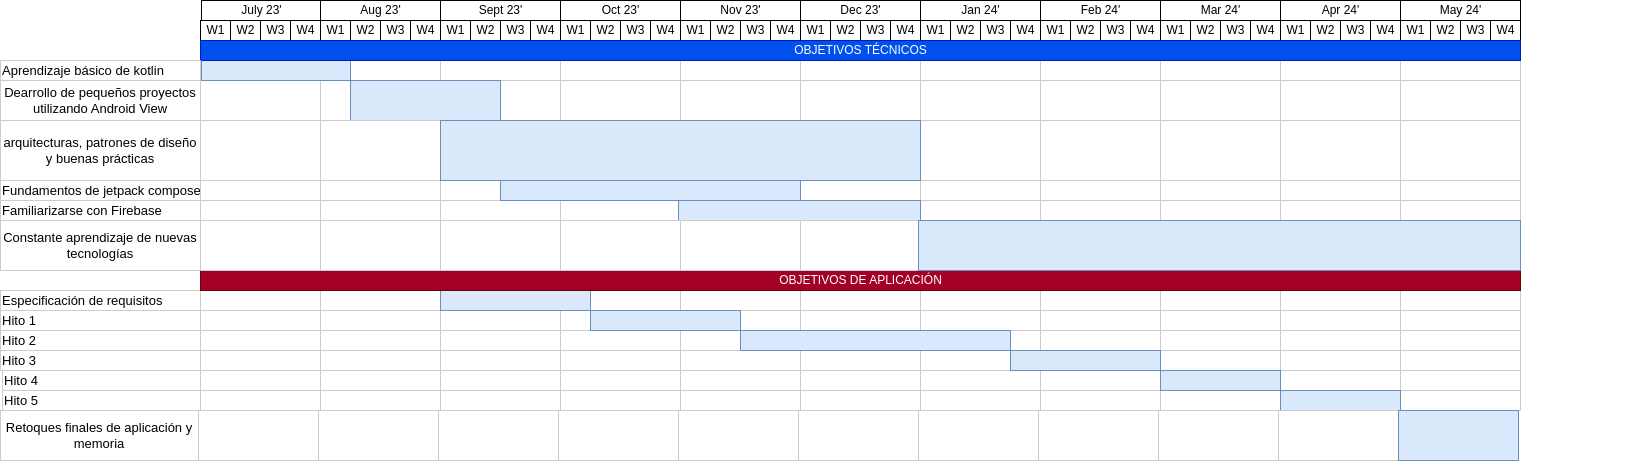
\includegraphics[width = 1\textwidth]{Imagenes/Bitmap/Gantt_Diagram.png}
	\caption{Diagrama de Gantt del proyecto}
	\label{fig:Gantt}
\end{figure}

Respecto a los hitos del proyecto, a continuación se muestra una lista con los casos de uso a desarrollar en cada hito:
\begin{itemize}
	\item Hito 1
	\begin{itemize}
		\item Registro/Baja de usuario.
		\item Modificar datos usuario.
		\item Login/Logout de usuario.
		\item Configurar app.
	\end{itemize}
	\item Hito 2
	\begin{itemize}
		\item Cambiar estado de profesional.
		\item Dar de alta/baja servicio.
		\item Modificar servicio.
		\item Listar servicios dados de alta.
		\item Añadir/Eliminar/Modificar categorías de servicios ofrecidos.
	\end{itemize}
	\item Hito 3
	\begin{itemize}
		\item Buscar servicio.
		\item Configurar búsqueda.
		\item Consultar profesional.
		\item Consultar cliente.
		\item Añadir/Quitar Profesional de lista de favoritos.
		\item Añadir/Modificar/Quitar cliente de lista de favoritos.
		\item Ver lista de favoritos.
	\end{itemize}
	\item Hito 4
	\begin{itemize}
		\item Contratar servicio.
		\item Chatear con profesional/cliente.
		\item Valorar cliente/profesional.
		\item Contestar solicitud de contratación.
	\end{itemize}
	\item Hito 5
	\begin{itemize}
		\item Consultar datos/estadísticas de profesional/clientes.
		\item Buscar clientes/profesionales.
		\item Modificar datos de clientes/profesionales/servicios ofrecidos.
		\item Dar de baja usuarios.
	\end{itemize}
\end{itemize}
Debido a que los casos de uso eran una aproximación inicial, según ha ido avanzando el proceso de desarrollo, algunos se han implementado antes, después, o se han descartado por no encajar bien en la aplicación. A pesar de esto, la planificación inicial, ha sido de gran utilidad como guía y ha servido para marcar correctamente los plazos de entrega, asimilando el proceso a como sería en un entorno real.
\chapter{Estado de la Cuestión}
\label{cap:estadoDeLaCuestion}

\section{Uber}
\begin{figure}[h]
	\centering
	
\includegraphics[width = 0.4\textwidth]{Imagenes/Fuentes/logo_Uber.png}
	\caption{Logotipo Uber}
	\label{fig:uber_logo}
\end{figure}
Uber \footnote{\url{https://www.uber.com}} es una aplicación muy conocida que sirve para contratar servicios de desplazamiento en V.T.C. (Vehículo de Transporte con Conductor), el motivo por el que se considera una aplicación relacionada con Profinder es que los servicios se contratan por proximidad, se utiliza la ubicación del usuario -al igual que se hace en Profinder- para encontrar los conductores más próximos, reduciendo así tiempos de espera y costes de desplazamiento innecesario. Uber se ha utilizado como una de las aplicaciones de referencia ya que representa muy bien el concepto que se ha buscado desde el principio con Profinder.

\section{Habitissimo}
\begin{figure}[h]
	\centering
	
\includegraphics[width = 0.4\textwidth]{Imagenes/Fuentes/habitissimo_logo.jpg}
	\caption{Logotipo Habitissimo}
	\label{fig:habitissimo_logo}
\end{figure}
Habitissimo \footnote{\url{https://www.habitissimo.es/}} es la posible competencia más directa que se ha encontrado. Es una aplicación en la que distintos profesionales pueden publicar ofertas de servicios, que los usuarios pueden contratar pidiendo un presupuesto. Esta aplicación está más enfocada a profesiones artesanales (carpintería, pintura, albañilería...) a diferencia de Profinder, que no está enfocada a ningún sector particular, sino que cuenta con distintas categorías que pueden ir ampliándose y ajustándose con el tiempo. Profinder también busca diferenciarse por tener un proceso más ágil que no dependa de ningún tipo de tercero y en el que se pueda tener un contacto más directo entre usuarios y profesionales. 

\section{Upwork}
\begin{figure}[h]
	\centering
	
\includegraphics[width = 0.4\textwidth]{Imagenes/Fuentes/logo_upwork.png}
	\caption{Logotipo Upwork}
	\label{fig:upwork_logo}
\end{figure}


\section{Booksy}
\begin{figure}[h]
	\centering
	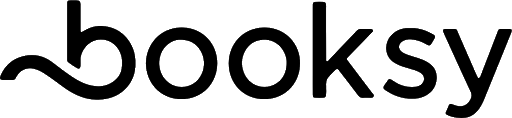
\includegraphics[width = 0.4\textwidth]{Imagenes/Fuentes/logo_booksy.png}
	\caption{Logotipo Booksy}
	\label{fig:booksy_logo}
\end{figure}
\chapter{Descripción del Trabajo}
\label{cap:descripcionTrabajo}

Aquí comienza la descripción del trabajo realizado. Se deben incluir tantos capítulos como sea necesario para describir de la manera más completa posible el trabajo que se ha llevado a cabo. Como muestra la figura, está todo por hacer.

\section{Tecnlogías empleadas}
\section{Justificación del diseño y consideraciones técnicas fundamentales}
\section{Modelo de datos}
%\include{Capitulos/Capitulo4}
%\include{Capitulos/Capitulo5}
\chapter{Conclusiones y Trabajo Futuro}
\label{cap:conclusiones}
En este capítulo han sido plasmadas las conclusiones, así como las posibles líneas de trabajo futuro del proyecto.
\section{Conclusiones}
Desde que se planteó este trabajo de fin de grado en Julio de 2023, hasta la fecha en que se están redactando estas conclusiones han pasado aproximadamente 11 meses. Ha sido un viaje en el que se partía prácticamente de cero en cuanto a concimientos específicos de Android y en el que no se han parado de aprender conceptos nuevos mes a mes, casi se ha convertido en un hábito el dedicar todo el tiempo libre posible al proyecto y como consecuencia ha quedado una aplicación completa a pesar de tener muchas cosas que mejorar y diversas líneas de trabajo a seguir para hacerlo más completo, al fin y al cabo, este aprendizaje constante es de lo que trata el mundo de la programación y el desarrollo de software. Y es esto precisamente lo que lo hace tan apasionante.

A nivel del código desarrollado, a medida que se han ido añadiendo funcionalidades se han encontrado multitud de cosas a mejorar, y se ha hecho en la medida de lo posible teniendo en cuenta los ajustados tiempos, a esto ha ayudado una base estructural robusta que ha hecho posible que el proceso de refactorización haya sido siempre cómodo y eficiente. Este proyecto ha servido también para entender lo importante que es hacer las cosas bien, en los proyectos iniciales, cuando era necesario hacer un cambio, el proceso se convertía en un infierno, cada cambio hacía que otras cosas no funcionaran y acababa siendo más fácil deshechar el cambio. Por eso se tomó la determinación de que se evitaría por todos los medios que esto pasara con Profinder. La elección de las tecnologías (como se ha descrito en el capítulo \ref{cap:tecnologiasEmpleadas}) también ha sido de vital importancia, esto se ha notado por ejemplo con el uso de \hyperlink{subsec:kotlin}{Kotlin} y \hyperlink{subsec:compose}{Jeptack Compose}.

Profinder ha conseguido cumplir los objetivos propuestos inicialmente: Una aplicación capaz de actuar como intermediario entre distintos tipos de expertos profesionales que busquen ofrecer un servicio y clientes dispuestos a consumirlo. Ofreciendo también una serie de funcionalidades que hagan del proceso anterior algo fluido, descentralizado y sin comisiones.

\section{Líneas de trabajo futuro}
Como se ha mencionado anteriormente, Profinder es una aplicación completa, sin embargo, hay múltitud de puntos en los que se podría mejorar y/o completar. A continuación se han mencionado algunos:
\begin{itemize}
    \item \textbf{Notificaciones}: añadiría un toque extra de calidad y personalización a la aplicación el uso de notificaciones, especialmente para funcionalidades como el chat (notificaciones cuando se envían y reciben mensajes), la solicitud de servicios o los trabajos (cuando emipecen y terminen).
    \item \textbf{Animaciones}: el uso de las animaciones en Android es otra de las cosas que añade calidad a las aplicaciones, en Profinder no ha dado tiempo ha implementarlas en su totalidad ya que son un campo muy ámplio, sí que se han usado en algunos casos puntuales (como el efecto Shimmer que es una animación, aunque para ello se ha utilizado una biblioteca externa\footnote{Repositorio de la bilioteca Shimmer realizada por el usuario valentinilk: \href{https://github.com/valentinilk/compose-shimmer}{compose-shimmer}.}) pero la intención a futuro sería implementarlas en muchas otras partes de la aplicación.
    \item \textbf{Testing}: Como se mencionó en el apartado \ref{subsec:testing}, el testing de la aplicación ha sido el reto más difícil a superar y por falta de tiempo se ha quedado un poco a medias, la idea sería hacer un ámplio sistema de tests que incluya test unitarios, de integración y de UI para aportar una mayor robustez y conseguir eliminar los \textit{bugs} que puedan ir surgiendo.
    \item \textbf{Refactor  \hyperlink{subsec:mvi}{MVI}}: a pesar de que el patrón \hyperlink{subsec:mvi}{MVI} se ha aplicado de una forma correcta en la aplicación, de cara al final del proyecto se ha descubierto que se han cometido algunos errores (también denominados antipatrones) que podrían afectar a la escalabilidad en el futuro, debido a esto una refactorización que arregle estos problemas sería una de las líneas de trabajo futuro.
    \item \textbf{Playstore}: En un inicio, se planteó la posibilidad de publicar la aplicación en la Playstore pero al final no se llevó a cabo debido a que antes de hacerlo entra en juego la seguridad del código, habría que seguir procesos de ofuscamiento, control de entornos y CI/CD. No ha dado tiempo a estudiar con la profundidad necesaria estos temas por lo que se ha clasificado como línea de trabajo futuro.
    \item \textbf{Rol de administrador}: En la especificación de requisitos inicial se declaró el administrador como un actor que gestionara la aplicación desde dentro de la misma, a lo largo del proyecto no se consideró de suficiente importancia dentro de los plazos y se decidió hacer más incapié en otras partes de la aplicación. Sin embargo, podría ser interesante darle una vuelta a este concepto para establecer un mejor control de usuarios dentro de la aplicación.
    \item \textbf{Hacerla multiplataforma}: \href{https://kotlinlang.org/docs/multiplatform.html}{Kotlin multiplatform} es una nueva forma de hacer aplicaciones usando \hyperlink{subsec:kotlin}{Kotlin} y \hyperlink{subsec:compose}{Jeptack Compose}, a día de hoy no es una tecnología suficientemente madura como para ser viable pero permitiria hacer aplicaciones para distintos sistemas operativos (IOS, Windows...) con la misma base de código, esto permitiría aumentar considerablemente el alcance de la aplicación y la haría más completa. No se descarta migrarla a Kotlin multiplatform en el futuro.
\end{itemize}




%%%%%%%%%%%%%%%%%%%%%%%%%%%%%%%%%%%%%%%%%%%%%%%%%%%%%%%%%%%%%%%%%%%%%%%%%%%
% Si el TFG se escribe en inglés, comentar las siguientes líneas 
% porque no es necesario incluir nuevamente las Conclusiones en inglés
\begin{otherlanguage}{english}
\chapter*{Introduction}
\label{cap:introduction}
\addcontentsline{toc}{chapter}{Introduction}

Introduction to the subject area. This chapter contains the translation of Chapter \ref{cap:introduccion}.










\chapter*{Conclusions and Future Work}
\label{cap:conclusions}
\addcontentsline{toc}{chapter}{Conclusions and Future Work}

Conclusions and future lines of work. This chapter contains the translation of Chapter \ref{cap:conclusiones}.



\end{otherlanguage}
%%%%%%%%%%%%%%%%%%%%%%%%%%%%%%%%%%%%%%%%%%%%%%%%%%%%%%%%%%%%%%%%%%%%%%%%%%%

% \chapter*{Contribuciones Personales}
\label{cap:contribucionesPersonales}
\addcontentsline{toc}{chapter}{Contribuciones Personales}

En caso de trabajos no unipersonales, cada participante indicará en la memoria su contribución al proyecto con una extensión de al menos dos páginas por cada uno de los participantes.

En caso de trabajo unipersonal, elimina esta página en el fichero \texttt{TFGTeXiS.tex} (comenta o borra la línea \verb|\chapter*{Contribuciones Personales}
\label{cap:contribucionesPersonales}
\addcontentsline{toc}{chapter}{Contribuciones Personales}

En caso de trabajos no unipersonales, cada participante indicará en la memoria su contribución al proyecto con una extensión de al menos dos páginas por cada uno de los participantes.

En caso de trabajo unipersonal, elimina esta página en el fichero \texttt{TFGTeXiS.tex} (comenta o borra la línea \verb|\chapter*{Contribuciones Personales}
\label{cap:contribucionesPersonales}
\addcontentsline{toc}{chapter}{Contribuciones Personales}

En caso de trabajos no unipersonales, cada participante indicará en la memoria su contribución al proyecto con una extensión de al menos dos páginas por cada uno de los participantes.

En caso de trabajo unipersonal, elimina esta página en el fichero \texttt{TFGTeXiS.tex} (comenta o borra la línea \verb|\include{Capitulos/ContribucionesPersonales}|).

\section*{Estudiante 1}
Al menos dos páginas con las contribuciones del estudiante 1.

\section*{Estudiante 2}
Al menos dos páginas con las contribuciones del estudiante 2. En caso de que haya más estudiantes, copia y pega una de estas secciones.

|).

\section*{Estudiante 1}
Al menos dos páginas con las contribuciones del estudiante 1.

\section*{Estudiante 2}
Al menos dos páginas con las contribuciones del estudiante 2. En caso de que haya más estudiantes, copia y pega una de estas secciones.

|).

\section*{Estudiante 1}
Al menos dos páginas con las contribuciones del estudiante 1.

\section*{Estudiante 2}
Al menos dos páginas con las contribuciones del estudiante 2. En caso de que haya más estudiantes, copia y pega una de estas secciones.



%
% Bibliografía
%
% Si el TFM se escribe en inglés, editar TeXiS/TeXiS_bib para cambiar el
% estilo de las referencias
%---------------------------------------------------------------------
%
%                      configBibliografia.tex
%
%---------------------------------------------------------------------
%
% bibliografia.tex
% Copyright 2009 Marco Antonio Gomez-Martin, Pedro Pablo Gomez-Martin
%
% This file belongs to the TeXiS manual, a LaTeX template for writting
% Thesis and other documents. The complete last TeXiS package can
% be obtained from http://gaia.fdi.ucm.es/projects/texis/
%
% Although the TeXiS template itself is distributed under the 
% conditions of the LaTeX Project Public License
% (http://www.latex-project.org/lppl.txt), the manual content
% uses the CC-BY-SA license that stays that you are free:
%
%    - to share & to copy, distribute and transmit the work
%    - to remix and to adapt the work
%
% under the following conditions:
%
%    - Attribution: you must attribute the work in the manner
%      specified by the author or licensor (but not in any way that
%      suggests that they endorse you or your use of the work).
%    - Share Alike: if you alter, transform, or build upon this
%      work, you may distribute the resulting work only under the
%      same, similar or a compatible license.
%
% The complete license is available in
% http://creativecommons.org/licenses/by-sa/3.0/legalcode
%
%---------------------------------------------------------------------
%
% Fichero  que  configura  los  parámetros  de  la  generación  de  la
% bibliografía.  Existen dos  parámetros configurables:  los ficheros
% .bib que se utilizan y la frase célebre que aparece justo antes de la
% primera referencia.
%
%---------------------------------------------------------------------


%%%%%%%%%%%%%%%%%%%%%%%%%%%%%%%%%%%%%%%%%%%%%%%%%%%%%%%%%%%%%%%%%%%%%%
% Definición de los ficheros .bib utilizados:
% \setBibFiles{<lista ficheros sin extension, separados por comas>}
% Nota:
% Es IMPORTANTE que los ficheros estén en la misma línea que
% el comando \setBibFiles. Si se desea utilizar varias líneas,
% terminarlas con una apertura de comentario.
%%%%%%%%%%%%%%%%%%%%%%%%%%%%%%%%%%%%%%%%%%%%%%%%%%%%%%%%%%%%%%%%%%%%%%
\setBibFiles{%
biblio%
}

%%%%%%%%%%%%%%%%%%%%%%%%%%%%%%%%%%%%%%%%%%%%%%%%%%%%%%%%%%%%%%%%%%%%%%
% Definición de la frase célebre para el capítulo de la
% bibliografía. Dentro normalmente se querrá hacer uso del entorno
% \begin{FraseCelebre}, que contendrá a su vez otros dos entornos,
% un \begin{Frase} y un \begin{Fuente}.
%
% Nota:
% Si no se quiere cita, se puede eliminar su definición (en la
% macro setCitaBibliografia{} ).
%%%%%%%%%%%%%%%%%%%%%%%%%%%%%%%%%%%%%%%%%%%%%%%%%%%%%%%%%%%%%%%%%%%%%%
\setCitaBibliografia{
\begin{FraseCelebre}
\begin{Frase}
  Nobody actually creates perfect code the first time around, except me. But there's only one of me.
\end{Frase}
\begin{Fuente}
  Linus Torwalds
\end{Fuente}
\end{FraseCelebre}
}


URLs referenciadas
\begin{itemize}
  \item \url{https://developer.android.com/studio/intro}
  \item \url{https://www.jetbrains.com/idea}
  \item \url{https://www.java.com}
  \item \url{https://www.scala-lang.org}
  \item \url{https://obsidian.md}
  \item \url{https://www.figma.com}
  \item \url{https://m3.material.io}
  \item \url{https://m3.material.io/styles/color/system/overview}
  \item \url{https://www.drawio.com/}
  \item \url{https://git-scm.com/}
  \item \url{https://github.com/}
  \item \url{https://github.com/jesseduffield/lazygit}
  \item \url{https://kotlinlang.org/}
  \item \url{https://www.plainconcepts.com/es/kotlin-android/}
  \item \url{https://www.fsf.org/}
  \item \url{https://www.gnu.org/}
  \item \url{https://www.mozilla.org/es-ES/firefox/}
  \item \url{https://neovim.io/}
  \item \url{https://www.linux.org/pages/}
  \item \url{https://developer.android.com/topic/libraries/architecture/viewmodel}
  \item \url{https://builtin.com/software-engineering-perspectives/mvvm-architecture}
  \item \url{https://developer.android.com/guide/components/intents-filters}
  \item \url{https://www.youtube.com/watch?v=MiLN2vs2Oe0}
  \item \url{https://kotlinlang.org/docs/control-flow.html#when-expression}
  \item \url{}
  \item \url{}
  \item \url{}
  \item \url{}
  \item \url{}
  \item \url{}
  \item \url{}
  \item \url{}
  \item \url{}
  \item \url{}
  \item \url{}
\end{itemize}

%%
%% Creamos la bibliografia
%%
\makeBib

% Variable local para emacs, para  que encuentre el fichero maestro de
% compilación y funcionen mejor algunas teclas rápidas de AucTeX

%%%
%%% Local Variables:
%%% mode: latex
%%% TeX-master: "../Tesis.tex"
%%% End:



% Apéndices
\appendix
\chapter{Especificación de requisitos}
\label{Appendix:srs}

En este apendice se especifican los actores y casos de uso de la aplicación Profinder. Se trata de una especificación inicial por lo que tanto actores como casos de uso han sido cambiados, ampliados o recortados a lo largo del proceso de desarrollo.

\section{Actores}
A continuación se describen los distintos actores de la aplicación:
\begin{itemize}
    \item \textbf{Usuario}: Un usuario es cualquier persona que se dé de alta como tal, debe haberse creado una cuenta e iniciado sesión para ser identificado, estos son los que contratan los servicios que los profesionales ofrecen, entre otras funciones los usuarios pueden ver el mapa de profesionales en tiempo real y filtrar los datos que le aparecen según la categoría de trabajo seleccionada.
    \item \textbf{Profesional}: Un profesional es cualquier persona que se dé de alta como tal, su proceso de registro es ligeramente diferente al de un usuario normal ya que deben especificar la categoría en la que son profesionales, así como otros detalles que sean importantes para su profesión.
    \item \textbf{Administrador}: El administrador de la aplicación es el que se encarga de la organización y el correcto funcionamiento de la misma, podrá añadir o eliminar categorías, bloquear usuarios y/o profesionales, así como responder a mensajes dirigidos a soporte, los administradores deben ser asignados una vez creada la cuenta desde fuera de la aplicación.
\end{itemize}
\section{Casos de Uso}
Los casos de uso se han clasificado en cuatro categorías según el actor principal del mismo.
\subsection{Índice de casos de uso}
\renewcommand{\labelenumii}{\theenumi.\arabic{enumii}.}
\begin{enumerate}
    \item Casos de uso generales
    \begin{enumerate}
        \item Registro/baja
        \item Modificar datos
        \item Login/logout
        \item Configurar app
        \item Ver lista de favoritos
        \item Valorar cliente/profesional
        \item Chatear con cliente/profesional
    \end{enumerate}
    \item Casos de uso de usuarios
    \begin{enumerate}
        \item Configurar búsqueda
        \item Buscar servicio
        \item Consultar profesional
        \item Contratar servicio
        \item Añadir/modificar/quitar profesional de lista de favoritos.
    \end{enumerate}
    \item Casos de uso de profesionales
    \begin{enumerate}
        \item Cambiar estado de profesional
        \item Dar de alta/baja servicio
        \item Modificar servicio
        \item Listar servicios dados de alta
        \item Contestar solicitud de contratación
        \item Consultar cliente
        \item Añadir/modificar/quitar cliente de lista de favoritos
    \end{enumerate}
    \item Casos de uso de administrador
    \begin{enumerate}
        \item Añadir/eliminar/modificar categorías de servicios ofrecidos.
        \item Consultar datos/estadísticas de profesional/clientes
        \item Buscar clientes/profesionales
        \item Modificar datos clientes/profesionales /servicios ofrecidos
        \item Dar de baja usuarios
    \end{enumerate}
\end{enumerate}
\newpage
\subsection{Casos de uso generales}
\begin{table}[!h]
	\begin{tabularx}{\textwidth}{|c|X|}
	\rowcolor[HTML]{00D2CB} 
	\hline          
	\textbf{Requisito} & \textbf{Registro/baja} \\
	\hline
	Identificador & 1.1 \\
	\hline
	Prioridad & Alta \\
	\hline
	Precondición & En caso de baja: tener una cuenta creada. \\
	\hline
	Descripción & Los actores de la aplicación tendrán que crear una cuenta para poder interactuar con la misma, así mismo tendrán la capacidad de dar de baja su cuenta cuando lo deseen. \\
	\hline
	Entrada & Nombre de usuario, correo electrónico, contraseña. \\
	\hline
	Salida & Actor registrado/dado de baja \\
	\hline
	Secuencia normal & \begin{tabular}{@{}p{1cm}|p{9.5cm}@{}}
		Paso & Acción \\
		\hline  
		1 & El actor abre la aplicación y se le muestra la pantalla para iniciar sesión con un botón específico para registrarse. \\
		\hline  
		2 & se selecciona la opción ‘Registrarse’. \\
		\hline  
		3 & El actor rellena el formulario con los datos de entrada y pulsa ‘Enviar’. \\
		\hline  
		4 & El sistema procesa el formulario y crea la cuenta. \\
		\end{tabular} \\
	\hline
	Postcondición & Se ha creado la cuenta. \\
	\hline
	Excepciones & \begin{tabular}{@{}p{1cm}|p{9.5cm}@{}}
		Paso & Acción \\
		\hline  
		4 & Los datos introducidos son incorrectos o no cumplen los requisitos. No se crea la cuenta y se avisa al usuario. \\
		\end{tabular}  \\
	\hline
	Comentarios & Este caso de uso permite registrar o dar de baja de la aplicación a actores de la misma. \\
	\hline
	Actores & Usuario, Profesional \\
	\hline            
	\end{tabularx}
	\caption{Registro/baja}
	\label{tab:cu_1}  
\end{table}

%---------------------------------------------------------------
\newpage
\begin{table}[!h]
	\begin{tabularx}{\textwidth}{|c|X|}
	\rowcolor[HTML]{00D2CB} 
	\hline          
	\textbf{Requisito} & \textbf{Modificar datos} \\
	\hline
	Identificador & 1.2 \\
	\hline
	Prioridad & Media \\
	\hline
	Precondición & Haber iniciado sesión. \\
	\hline
	Descripción & Una vez creada una cuenta, tanto profesionales como usuarios podrán modificar sus datos de perfil. \\
	\hline
	Entrada & Datos a cambiar. \\
	\hline
	Salida & Nuevos datos. \\
	\hline
	Secuencia normal & \begin{tabular}{@{}p{1cm}|p{9.5cm}@{}}
		Paso & Acción \\
		\hline  
		1 & El actor se dirigirá al apartado de 'Mi perfil' y seleccionará la opción 'Modificar perfil'. \\
		\hline  
		2 & Dentro de esta pantalla se modificarán todos los datos deseados. \\
		\end{tabular} \\
	\hline
	Postcondición & Se han modificado los datos de perfil deseados. \\
	\hline
	Excepciones & \begin{tabular}{@{}p{1cm}|p{9.5cm}@{}}
		Paso & Acción \\
		\hline  
		2 & Los nuevos datos no son válidos. No se guarda la modificación. \\
		\end{tabular}  \\
	\hline
	Comentarios & Este caso de uso permite modificar datos de su perfil a los actores. \\
	\hline
	Actores & Usuario, Profesional \\
	\hline            
	\end{tabularx}
	\caption{Modificar datos}
	\label{tab:cu_2}  
\end{table}

%---------------------------------------------------------------
\begin{table}[tbph]
	\begin{tabularx}{\textwidth}{|c|X|}
	\rowcolor[HTML]{00D2CB} 
	\hline          
	\textbf{Requisito} & \textbf{Login/Logout} \\
	\hline
	Identificador & 1.3 \\
	\hline
	Prioridad & Alta \\
	\hline
	Precondición & Haber creado una cuenta previamente, en caso de logout tener sesión iniciada. \\
	\hline
	Descripción & Para poder interactuar con la aplicación, tanto usuarios como profesionales tendrán que iniciar sesión en la aplicación. Los usuarios que ya hayan iniciado sesión y quieran cerrarla tendrán la opción de hacerlo. \\
	\hline
	Entrada & En caso de login: correo electrónico/nombre de usuario, contraseña. \\
	\hline
	Salida & N.A. \\
	\hline
	Secuencia normal de login & \begin{tabular}{@{}p{1.5cm}|p{7.2cm}@{}}
		Paso & Acción \\
		\hline  
		1 & El actor abre la aplicación y se le muestra la pantalla de  ‘Iniciar sesión’. \\
		\hline  
		2 & Se muestra una pantalla con el formulario de inicio de sesión. El usuario introduce los datos de entrada y pulsa el botón ‘Iniciar sesión’. \\
		\end{tabular} \\
	\hline
	Secuencia normal de logout & \begin{tabular}{@{}p{1.5cm}|p{7.2cm}@{}}
		Paso & Acción \\
		\hline  
		1 & El actor se dirige a la sección ‘Mi perfil’ donde se le mostrarán múltiples opciones de gestión de su cuenta. \\
		\hline  
		2 & Dentro de estas opciones se encontrará la opción ‘Cerrar sesión’. El actor pulsará el botón. \\
		\end{tabular} \\
	\hline
	Postcondición & Se ha iniciado sesión/se ha cerrado sesión. \\
	\hline
	Excepciones & \begin{tabular}{@{}p{1.5cm}|p{7.2cm}@{}}
		Paso & Acción \\
		\hline  
		2 (login) & Los campos rellenados no concuerdan con ningún actor del sistema. No se completa el login. \\
		\end{tabular}  \\
	\hline
	Comentarios & Este caso de uso permite iniciar sesión en la aplicación, así como cerrar la misma. \\
	\hline
	Actores & Usuario, Profesional, Administrador \\
	\hline            
	\end{tabularx}
	\caption{Login/Logout}
	\label{tab:cu_3}  
\end{table}
%---------------------------------------------------------------
\newpage
\begin{table}[!h]
	\begin{tabularx}{\textwidth}{|c|X|}
	\rowcolor[HTML]{00D2CB} 
	\hline          
	\textbf{Requisito} & \textbf{Configurar app} \\
	\hline
	Identificador & 1.4 \\
	\hline
	Prioridad & Baja \\
	\hline
	Precondición & Haber iniciado sesión. \\
	\hline
	Descripción & Dentro de la app se podrán configurar aspectos como el tema de la aplicación (claro/oscuro). \\
	\hline
	Entrada & Nuevos datos de configuración. \\
	\hline
	Salida & Configuración modificada. \\
	\hline
	Secuencia normal & \begin{tabular}{@{}p{1cm}|p{9.5cm}@{}}
		Paso & Acción \\
		\hline  
		1 & El actor se dirigirá a la sección de ‘Mi Perfil’ y entre las opciones seleccionará ‘Configuración de la aplicación’. \\
		\hline  
		2 & Dentro de esta pantalla el usuario cambiará los valores deseados. \\
		\end{tabular} \\
	\hline
	Postcondición & Se han cambiado los parámetros de la aplicación deseados. \\
	\hline
	Excepciones & \begin{tabular}{@{}p{1cm}|p{9.5cm}@{}}
		Paso & Acción \\
		\hline  
		2 & Los nuevos parámetros de configuración no son correctos. Se mantiene la configuración anterior. \\
		\end{tabular}  \\
	\hline
	Comentarios & Este caso de uso permite modificar la configuración de la aplicación. \\
	\hline
	Actores & Usuario, Profesional \\
	\hline            
	\end{tabularx}
	\caption{Configurar app}
	\label{tab:cu_4}  
\end{table}

%---------------------------------------------------------------
\newpage
\begin{table}[!h]
	\begin{tabularx}{\textwidth}{|c|X|}
	\rowcolor[HTML]{00D2CB} 
	\hline          
	\textbf{Requisito} & \textbf{Ver lista de favoritos} \\
	\hline
	Identificador & 1.5 \\
	\hline
	Prioridad & Media \\
	\hline
	Precondición & El Usuario o Profesional debe estar autenticado en la aplicación y tener al menos un elemento en su lista de favoritos. \\
	\hline
	Descripción & Permite al Usuario o Profesional ver la lista de elementos marcados como favoritos (por ejemplo, Clientes o Profesionales) para un acceso rápido y conveniente. \\
	\hline
	Entrada & Selección de la opción para ver la lista de favoritos. \\
	\hline
	Salida & Lista de elementos marcados como favoritos con detalles relevantes. \\
	\hline
	Secuencia normal & \begin{tabular}{@{}p{1cm}|p{9.5cm}@{}}
		Paso & Acción \\
		\hline  
		1 & El Usuario o Profesional accede a la sección de lista de favoritos. \\
		\hline  
		2 & Selecciona la opción para ver la lista de favoritos. \\
		\hline  
		3 & Visualiza la lista de elementos marcados como favoritos con sus detalles. \\
		\end{tabular} \\
	\hline
	Postcondición & El Usuario o Profesional ve la lista de elementos marcados como favoritos. \\
	\hline
	Excepciones & \begin{tabular}{@{}p{1cm}|p{9.5cm}@{}}
		Paso & Acción \\
		\hline  
		2 & Si la lista de favoritos está vacía, se muestra un mensaje indicando que no hay elementos en la lista. \\
		\end{tabular}  \\
	\hline
	Comentarios & N.A. \\
	\hline
	Actores & Usuario, profesional \\
	\hline            
	\end{tabularx}
	\caption{Ver lista de favoritos}
	\label{tab:cu_5}  
\end{table}

%---------------------------------------------------------------
\newpage
\begin{table}[!h]
	\begin{tabularx}{\textwidth}{|c|X|}
	\rowcolor[HTML]{00D2CB} 
	\hline          
	\textbf{Requisito} & \textbf{Valorar cliente/profesional} \\
	\hline
	Identificador & 1.6 \\
	\hline
	Prioridad & Alta \\
	\hline
	Precondición & Haber iniciado sesión, haber recibido el trabajo de un profesional o haber realizado un trabajo a un usuario. \\
	\hline
	Descripción & Una vez realizado/recibido un trabajo, los usuarios/profesionales podrán valorar a ese profesional/usuario así como denunciarlo si lo vieran necesario. \\
	\hline
	Entrada & Datos de valoración, mensaje con más detalles (opcional) \\
	\hline
	Salida & N.A. \\
	\hline
	Secuencia normal & \begin{tabular}{@{}p{1cm}|p{9.5cm}@{}}
		Paso & Acción \\
		\hline  
		1 & Una vez recibido/realizado el trabajo, se mostrará la opción de valorar al profesional/usuario. \\
		\hline  
		2 & El usuario/profesional rellena el formulario de valoración. \\
		\end{tabular} \\
	\hline
	Postcondición & Se ha valorado al profesional/usuario. \\
	\hline
	Excepciones & \begin{tabular}{@{}p{1cm}|p{9.5cm}@{}}
		Paso & Acción \\
		\hline  
		2 & Los datos de entrada no son correctos. No se completa la valoración. \\
		\end{tabular}  \\
	\hline
	Comentarios & N.A. \\
	\hline
	Actores & Usuario, profesional \\
	\hline            
	\end{tabularx}
	\caption{Valorar cliente/profesional}
	\label{tab:cu_6}  
\end{table}

%---------------------------------------------------------------
\newpage
\begin{table}[!h]
	\begin{tabularx}{\textwidth}{|c|X|}
	\rowcolor[HTML]{00D2CB} 
	\hline          
	\textbf{Requisito} & \textbf{Chatear con cliente/profesional} \\
	\hline
	Identificador & 1.7 \\
	\hline
	Prioridad & Media \\
	\hline
	Precondición & Haber iniciado sesión, estar en el perfil de un profesional/cliente. \\
	\hline
	Descripción & En el perfil de los profesionales/clientes habrá un botón para iniciar un chat privado que servirá para aclarar dudas, pedir/dar presupuestos para cosas concretas, etc…  \\
	\hline
	Entrada & botón de chat, mensaje(s) a enviar. \\
	\hline
	Salida & N.A. \\
	\hline
	Secuencia normal & \begin{tabular}{@{}p{1cm}|p{9.5cm}@{}}
		Paso & Acción \\
		\hline  
		1 & Una vez en el perfil del profesional/usuario se pulsa el botón ‘Chat privado’. \\
		\hline  
		2 & Al hacerlo, se abre un chat entre usuario y profesional donde se podrán enviar mensajes. \\
		\hline  
		3 & El usuario/profesional envía los mensajes deseados. \\
		\end{tabular} \\
	\hline
	Postcondición & Se ha creado un chat privado entre usuario y profesional. \\
	\hline
	Excepciones & N.A.\\
	\hline
	Comentarios & Este caso de uso permite establecer una conversación entre usuario y profesional. \\
	\hline
	Actores & Usuario, profesional \\
	\hline            
	\end{tabularx}
	\caption{Chatear con profesional}
	\label{tab:cu_7}  
\end{table}

\newpage
\subsection{Casos de uso de usuarios}

\begin{table}[!h]
	\begin{tabularx}{\textwidth}{|c|X|}
	\rowcolor[HTML]{00D2CB} 
	\hline          
	\textbf{Requisito} & \textbf{Configurar búsqueda} \\
	\hline
	Identificador & 2.1 \\
	\hline
	Prioridad & Media \\
	\hline
	Precondición & Haber iniciado sesión. \\
	\hline
	Descripción & A la hora de buscar el servicio de un profesional, los usuarios tendrán la opción de configurar los parámetros de la búsqueda como por ejemplo, seleccionar una categoría u ordenar por valoración. \\
	\hline
	Entrada & Datos de configuración de búsqueda. \\
	\hline
	Salida & N.A. \\
	\hline
	Secuencia normal & \begin{tabular}{@{}p{1cm}|p{9.5cm}@{}}
		Paso & Acción \\
		\hline  
		1 & Dentro de la aplicación, el usuario seleccionará la opción ‘Buscar profesional’. \\
		\hline  
		2 & Se configurarán todos los parámetros de la búsqueda y se pulsará el botón ‘Buscar’. \\
		\end{tabular} \\
	\hline
	Postcondición & Se han configurado los parámetros de la búsqueda. \\
	\hline
	Excepciones & N.A.  \\
	\hline
	Comentarios & Este caso de uso permite establecer unos parámetros determinados de búsqueda. \\
	\hline
	Actores & Usuario \\
	\hline            
	\end{tabularx}
	\caption{Configurar búsqueda}
	\label{tab:cu_8}  
\end{table}

%---------------------------------------------------------------
\newpage
\begin{table}[!h]
	\begin{tabularx}{\textwidth}{|c|X|}
	\rowcolor[HTML]{00D2CB} 
	\hline          
	\textbf{Requisito} & \textbf{Buscar servicio} \\
	\hline
	Identificador & 2.2 \\
	\hline
	Prioridad & Media \\
	\hline
	Precondición & Haber iniciado sesión, haber configurado la búsqueda. \\
	\hline
	Descripción & Una vez configurados los parámetros de búsqueda, se mostrarán los servicios que cumplen los parámetros de la búsqueda para que el usuario pueda realizar la búsqueda.  \\
	\hline
	Entrada & Servicio a buscar. \\
	\hline
	Salida & Resultados de servicios que coinciden con la búsqueda. \\
	\hline
	Secuencia normal & \begin{tabular}{@{}p{1cm}|p{9.5cm}@{}}
		Paso & Acción \\
		\hline  
		1 & El usuario podrá recorrer una lista con todos los servicios ofrecidos que cumplen los filtros establecidos. \\
		\end{tabular} \\
	\hline
	Postcondición & Se ha realizado una búsqueda de servicio. \\
	\hline
	Excepciones & N.A.\\
	\hline
	Comentarios & Este caso de uso sirve para que los usuarios puedan buscar servicios de acuerdo con unos parámetros \\
	\hline
	Actores & Usuario \\
	\hline            
	\end{tabularx}
	\caption{Buscar servicio}
	\label{tab:cu_9}  
\end{table}

%---------------------------------------------------------------
\newpage
\begin{table}[!h]
	\begin{tabularx}{\textwidth}{|c|X|}
	\rowcolor[HTML]{00D2CB} 
	\hline          
	\textbf{Requisito} & \textbf{Consultar profesional} \\
	\hline
	Identificador & 2.3 \\
	\hline
	Prioridad & Media \\
	\hline
	Precondición & Haber iniciado sesión, Hay profesionales disponibles. \\
	\hline
	Descripción & Los usuarios tendrán la posibilidad de consultar el perfil de los distintos profesionales: sus datos (categoría, honorarios, etc…), sus valoraciones y otras estadísticas.  \\
	\hline
	Entrada & Profesional a consultar. \\
	\hline
	Salida & Detalles del profesional consultado \\
	\hline
	Secuencia normal & \begin{tabular}{@{}p{1cm}|p{9.5cm}@{}}
		Paso & Acción \\
		\hline  
		1 & El usuario realiza una búsqueda de profesional o escoge uno de los que se muestra en el mapa. \\
		\hline  
		2 & Al pulsar en el profesional se abrirá su perfil con todos los datos de ese profesional. \\
		\end{tabular} \\
	\hline
	Postcondición & Se ha consultado el profesional seleccionado. \\
	\hline
	Excepciones & N.A.\\
	\hline
	Comentarios & Este caso de uso permite obtener más detalles acerca de un profesional determinado. \\
	\hline
	Actores & Usuario \\
	\hline            
	\end{tabularx}
	\caption{Chatear con profesional}
	\label{tab:cu_10}  
\end{table}

%---------------------------------------------------------------
\newpage
\begin{table}[!h]
	\begin{tabularx}{\textwidth}{|c|X|}
	\rowcolor[HTML]{00D2CB} 
	\hline          
	\textbf{Requisito} & \textbf{Contratar servicio} \\
	\hline
	Identificador & 2.4 \\
	\hline
	Prioridad & Alta \\
	\hline
	Precondición & Haber iniciado sesión. \\
	\hline
	Descripción & Cuando un usuario encuentre el servicio que necesita tendrá la posibilidad de contratarlo y el profesional decidirá si tomar o no el trabajo.  \\
	\hline
	Entrada & Servicio elegido, respuesta del profesional. \\
	\hline
	Salida & N.A. \\
	\hline
	Secuencia normal & \begin{tabular}{@{}p{1cm}|p{9.5cm}@{}}
		Paso & Acción \\
		\hline  
		1 & Una vez seleccionado el profesional, en la pantalla del perfil del mismo habrá una opción llamada ‘Contratar servicio’, el usuario pulsará el botón. \\
		\hline  
		2 & El sistema procesa y valida la contratación. \\
		\hline  
		3 & La propuesta de trabajo llega al profesional que decide si la acepta o rechaza. \\
		\end{tabular} \\
	\hline
	Postcondición & Se ha contratado el servicio. \\
	\hline
	Excepciones & \begin{tabular}{@{}p{1cm}|p{9.5cm}@{}}
		Paso & Acción \\
		2 & Fallo en el proceso y validación de la petición. Se avisa al usuario y no se envía la propuesta. \\
		\end{tabular}\\
	\hline
	Comentarios & N.A. \\
	\hline
	Actores & Usuario \\
	\hline            
	\end{tabularx}
	\caption{Contratar servicio}
	\label{tab:cu_11}  
\end{table}

%---------------------------------------------------------------
\newpage
\begin{table}[!h]
	\begin{tabularx}{\textwidth}{|c|X|}
	\rowcolor[HTML]{00D2CB} 
	\hline          
	\textbf{Requisito} & \textbf{Añadir/Quitar Profesional de lista de favoritos} \\
	\hline
	Identificador & 2.5 \\
	\hline
	Prioridad & Media \\
	\hline
	Precondición & Haber iniciado sesión, estar en el perfil de un profesional. \\
	\hline
	Descripción & Los usuarios tendrán la posibilidad de añadir o quitar a profesionales de su lista de favoritos, lista en la que podrán tener un acceso rápido a los perfiles de dichos profesionales.  \\
	\hline
	Entrada & Botón de añadir/quitar de favoritos. \\
	\hline
	Salida & Lista de favoritos modificada. \\
	\hline
	Secuencia normal & \begin{tabular}{@{}p{1cm}|p{9.5cm}@{}}
		Paso & Acción \\
		\hline  
		1 & Una vez dentro del perfil de un profesional, el usuario dispondrá de un botón de favoritos. \\
		\hline  
		2 & Dependiendo de si quiere añadir o quitar al profesional de favorito lo activará o desactivará. \\
		\end{tabular} \\
	\hline
	Postcondición & Se ha añadido/quitado un profesional en la lista de favoritos. \\
	\hline
	Excepciones & N.A.\\
	\hline
	Comentarios & N.A. \\
	\hline
	Actores & Usuario \\
	\hline            
	\end{tabularx}
	\caption{Contratar servicio}
	\label{tab:cu_12}  
\end{table}
%---------------------------------------------------------------
\newpage
\subsection{Casos de uso de profesionales}
\begin{table}[!h]
	\begin{tabularx}{\textwidth}{|c|X|}
	\rowcolor[HTML]{00D2CB} 
	\hline          
	\textbf{Requisito} & \textbf{Cambiar estado de profesional} \\
	\hline
	Identificador & 3.1 \\
	\hline
	Prioridad & Alta \\
	\hline
	Precondición & Haber iniciado sesión como profesional. \\
	\hline
	Descripción & El profesional puede cambiar su estado entre activo/inactivo/trabajando para indicar a los usuarios su disponibilidad actual. \\
	\hline
	Entrada & Nuevo estado. \\
	\hline
	Salida & N.A. \\
	\hline
	Secuencia normal & \begin{tabular}{@{}p{1cm}|p{9.5cm}@{}}
		Paso & Acción \\
		\hline  
		1 & El profesional se dirige al apartado de ‘Mi Perfil’. \\
		\hline  
		2 & Dentro del mismo selecciona la opción ‘Cambiar estado’. \\
		\hline  
		3 & El profesional selecciona el nuevo estado que figura en su perfil. \\
		\end{tabular} \\
	\hline
	Postcondición & Se ha cambiado el estado de profesional. \\
	\hline
	Excepciones & N.A. \\
	\hline
	Comentarios & N.A. \\
	\hline
	Profesional   \\
	\hline            
	\end{tabularx}
	\caption{Cambiar estado de profesional}
	\label{tab:cu_13}  
\end{table}

%---------------------------------------------------------------
\newpage
\begin{table}[!h]
	\begin{tabularx}{\textwidth}{|c|X|}
	\rowcolor[HTML]{00D2CB} 
	\hline          
	\textbf{Requisito} & \textbf{Dar de alta/baja servicio} \\
	\hline
	Identificador & 3.2 \\
	\hline
	Prioridad & Alta \\
	\hline
	Precondición & Haber iniciado sesión como profesional. \\
	\hline
	Descripción & Los profesionales tendrán la opción de dar de alta y baja los servicios, en el primer caso esto significa que sube un servicio y en el segundo que retira de la oferta de servicios. \\
	\hline
	Entrada & Servicio a dar de baja/alta. \\
	\hline
	Salida & Confirmación de la baja/alta del servicio. \\
	\hline
	Secuencia normal: alta de servicio & \begin{tabular}{@{}p{1cm}|p{6.5cm}@{}}
		Paso & Acción \\
		\hline  
		1 & Cuando un usuario contrata el servicio de un profesional, a este le llega una solicitud de servicio. \\
		\hline  
		2 & El profesional abre la oferta, donde verá los detalles del servicio. \\
		\hline  
		3 & Pulsa el botón ‘Aceptar servicio’. \\
		\end{tabular} \\
	\hline
	Secuencia normal: baja de servicio & \begin{tabular}{@{}p{1cm}|p{6.5cm}@{}}
		Paso & Acción \\
		\hline  
		1 & El profesional abre el servicio que había aceptado con anterioridad. \\
		\hline  
		2 & Entre los detalles del servicio se muestra la opción ‘Dar de baja servicio’ el profesional pulsa el botón. \\
		\hline  
		3 & Se muestra un mensaje de confirmación de baja de servicio. \\
		\end{tabular} \\
	\hline
	Postcondición & Se ha dado de alta/baja un servicio. \\
	\hline
	Excepciones & N.A.  \\
	\hline
	Comentarios & N.A. \\
	\hline
	Actores & Profesional   \\
	\hline            
	\end{tabularx}
	\caption{Dar de alta/baja servicio}
	\label{tab:cu_14}  
\end{table}

%---------------------------------------------------------------
\newpage
\begin{table}[!h]
	\begin{tabularx}{\textwidth}{|c|X|}
	\rowcolor[HTML]{00D2CB} 
	\hline          
	\textbf{Requisito} & \textbf{Modificar servicio} \\
	\hline
	Identificador & 3.3 \\
	\hline
	Prioridad & Alta \\
	\hline
	Precondición & Haber iniciado sesión como profesional, tener al menos un servicio dado de alta. \\
	\hline
	Descripción & Permite al Profesional modificar la información de un servicio que ofrece. \\
	\hline
	Entrada & Detalles actualizados del servicio. \\
	\hline
	Salida & Confirmación de la modificación del servicio. \\
	\hline
	Secuencia normal & \begin{tabular}{@{}p{1cm}|p{9.5cm}@{}}
		Paso & Acción \\
		\hline  
		1 & El profesional navega hasta la sección de gestión de servicios. \\
		\hline  
		2 & Selecciona el servicio que desea modificar. \\
		\hline  
		3 & Realiza las modificaciones necesarias en los detalles del servicio. \\
		\hline  
		4 & Confirma la acción de modificación. \\
		\end{tabular} \\
	\hline
	Postcondición & El servicio se actualiza con la nueva información en el perfil del Profesional. \\
	\hline
	Excepciones & \begin{tabular}{@{}p{1cm}|p{9.5cm}@{}}
		Paso & Acción \\
		\hline  
		3 & Si no se proporciona la información necesaria, se muestra un mensaje de error. \\
		\hline  
		4 & Si la operación falla por algún motivo, se notifica al Profesional. \\
		\end{tabular}  \\
	\hline
	Comentarios & Este caso de uso permite a los Profesionales mantener actualizada la información de sus servicios. \\
	\hline
	Actores & Profesional   \\
	\hline            
	\end{tabularx}
	\caption{Modificar servicio}
	\label{tab:cu_15}  
\end{table}

%---------------------------------------------------------------
\newpage
\begin{table}[!h]
	\begin{tabularx}{\textwidth}{|c|X|}
	\rowcolor[HTML]{00D2CB} 
	\hline          
	\textbf{Requisito} & \textbf{Listar servicios dados de alta} \\
	\hline
	Identificador & 3.4 \\
	\hline
	Prioridad & Baja \\
	\hline
	Precondición & Haber iniciado sesión como profesional, tener al menos un servicio dado de alta. \\
	\hline
	Descripción & Permite al Profesional ver una lista de todos los servicios que ha dado de alta. \\
	\hline
	Entrada & Selección de la opción para listar servicios. \\
	\hline
	Salida & Lista de servicios con detalles. \\
	\hline
	Secuencia normal & \begin{tabular}{@{}p{1cm}|p{9.5cm}@{}}
		Paso & Acción \\
		\hline  
		1 & El profesional navega hasta la sección de gestión de servicios. \\
		\hline  
		2 & Selecciona la opción para listar sus servicios. \\
		\end{tabular} \\
	\hline
	Postcondición & El Profesional puede ver una lista de los servicios que ha dado de alta. \\
	\hline
	Excepciones & \begin{tabular}{@{}p{1cm}|p{9.5cm}@{}}
		Paso & Acción \\
		\hline  
		2 & Si no tiene servicios dados de alta, se muestra un mensaje indicando que no tiene servicios registrados. \\
		\end{tabular}  \\
	\hline
	Comentarios & N.A. \\
	\hline
	Actores & Profesional   \\
	\hline            
	\end{tabularx}
	\caption{Listar servicios dados de alta}
	\label{tab:cu_16}  
\end{table}

%---------------------------------------------------------------
\newpage
\begin{table}[!h]
	\begin{tabularx}{\textwidth}{|c|X|}
	\rowcolor[HTML]{00D2CB} 
	\hline          
	\textbf{Requisito} & \textbf{Contestar solicitud de contratación.} \\
	\hline
	Identificador & 3.5 \\
	\hline
	Prioridad & Alta \\
	\hline
	Precondición & El Profesional debe estar autenticado en la aplicación y haber recibido una solicitud de contratación. \\
	\hline
	Descripción & Permite al Profesional aceptar o rechazar una solicitud de contratación de un Usuario. \\
	\hline
	Entrada & Solicitud de contratación. \\
	\hline
	Salida & Confirmación de la respuesta a la solicitud. \\
	\hline
	Secuencia normal & \begin{tabular}{@{}p{1cm}|p{9.5cm}@{}}
		Paso & Acción \\
		\hline  
		1 & El profesional recibe una notificación de solicitud de contratación. \\
		\hline  
		2 & Accede a la solicitud y selecciona aceptar o rechazar. \\
		\hline  
		3 & Confirma la respuesta. \\
		\end{tabular} \\
	\hline
	Postcondición & La solicitud de contratación se responde y se notifica al Usuario. \\
	\hline
	Excepciones & \begin{tabular}{@{}p{1cm}|p{9.5cm}@{}}
		Paso & Acción \\
		\hline  
		3 & Si la solicitud ha caducado, se informa al Profesional. \\
		\end{tabular}  \\
	\hline
	Comentarios & N.A. \\
	\hline
	Actores & Usuario, Profesional   \\
	\hline            
	\end{tabularx}
	\caption{Contestar solicitud de contratación.}
	\label{tab:cu_17}  
\end{table}

%---------------------------------------------------------------
\newpage
\begin{table}[!h]
	\begin{tabularx}{\textwidth}{|c|X|}
	\rowcolor[HTML]{00D2CB} 
	\hline          
	\textbf{Requisito} & \textbf{Consultar cliente} \\
	\hline
	Identificador & 3.6 \\
	\hline
	Prioridad & Media \\
	\hline
	Precondición & Haber iniciado sesión como profesional y estar trabajando o haber trabajado con el cliente. \\
	\hline
	Descripción & Permite al Profesional consultar información sobre el cliente, incluyendo sus datos, las valoraciones que ha recibido y otras estadísticas relevantes. \\
	\hline
	Entrada & Selección del Cliente a consultar. \\
	\hline
	Salida & Información detallada del Cliente, incluyendo sus datos personales, valoraciones recibidas y estadísticas. \\
	\hline
	Secuencia normal & \begin{tabular}{@{}p{1cm}|p{9.5cm}@{}}
		Paso & Acción \\
		\hline  
		1 & El profesional accede a la sección de consulta de Clientes. \\
		\hline  
		2 & Selecciona el Cliente cuya información desea consultar. \\
		\hline  
		3 & Visualiza los datos y estadísticas del cliente. \\
		\end{tabular} \\
	\hline
	Postcondición & El Profesional obtiene información sobre el cliente. \\
	\hline
	Excepciones & N.A.\\
	\hline
	Comentarios & Este caso de uso brinda al Profesional acceso a información relevante sobre los Clientes con los que ha interactuado. \\
	\hline
	Actores & Usuario, Profesional \\
	\hline            
	\end{tabularx}
	\caption{Consultar cliente.}
	\label{tab:cu_18}  
\end{table}

%---------------------------------------------------------------
\newpage
\begin{table}[!h]
	\begin{tabularx}{\textwidth}{|c|X|}
	\rowcolor[HTML]{00D2CB} 
	\hline          
	\textbf{Requisito} & \textbf{Añadir/Modificar/Quitar cliente de lista de favoritos.} \\
	\hline
	Identificador & 3.7 \\
	\hline
	Prioridad & Media \\
	\hline
	Precondición & Haber iniciado sesión como profesional. \\
	\hline
	Descripción & Permite al Profesional agregar, modificar o quitar Clientes de su lista de favoritos para un acceso más rápido y conveniente. \\
	\hline
	Entrada & Selección de la acción (añadir, modificar o quitar) y Cliente seleccionado. \\
	\hline
	Salida & N.A. \\
	\hline
	Secuencia normal & \begin{tabular}{@{}p{1cm}|p{9.5cm}@{}}
		Paso & Acción \\
		\hline  
		1 & El profesional navega hasta la sección de gestión de favoritos. \\
		\hline  
		2 & Selecciona la acción deseada (añadir, modificar o quitar) y el cliente correspondiente. \\
		\hline  
		3 & Confirma la acción. \\
		\end{tabular} \\
	\hline
	Postcondición & La lista de favoritos se actualiza según la acción realizada. \\
	\hline
	Excepciones & \begin{tabular}{@{}p{1cm}|p{9.5cm}@{}}
		Paso & Acción \\
		\hline  
		2 & Si el Cliente ya está en la lista de favoritos y se selecciona "añadir", se muestra un mensaje informativo. \\
		\end{tabular}  \\
	\hline
	Comentarios & Este caso de uso permite al Profesional gestionar su lista de favoritos para un acceso más rápido a los Clientes preferidos. \\
	\hline
	Actores & Usuario, Profesional   \\
	\hline            
	\end{tabularx}
	\caption{Añadir/Modificar/Quitar cliente de lista de favoritos.}
	\label{tab:cu_19}  
\end{table}

\newpage
\subsection{Casos de uso de administrador}

\begin{table}[!h]
	\begin{tabularx}{\textwidth}{|c|X|}
	\rowcolor[HTML]{00D2CB} 
	\hline          
	\textbf{Requisito} & \textbf{Añadir/eliminar/Modificar categorías de servicios ofrecidos.} \\
	\hline
	Identificador & 4.1 \\
	\hline
	Prioridad & Alta \\
	\hline
	Precondición & Estar registrado en la aplicación como administrador. \\
	\hline
	Descripción & Permite al Administrador gestionar las categorías de servicios ofrecidos, incluyendo la adición, eliminación o modificación de categorías existentes. \\
	\hline
	Entrada & Selección de la acción (añadir, eliminar o modificar) y detalles de la categoría. \\
	\hline
	Salida & Confirmación de la acción realizada en las categorías. \\
	\hline
	Secuencia normal & \begin{tabular}{@{}p{1cm}|p{9.5cm}@{}}
		Paso & Acción \\
		\hline  
		1 & El administrador accede a la sección de gestión de categorías de servicios. \\
		\hline  
		2 & Selecciona la acción deseada (añadir, eliminar o modificar) y proporciona los detalles necesarios. \\
		\hline  
		3 & Confirma la acción. \\
		\end{tabular} \\
	\hline
	Postcondición & Las categorías se actualizan según la acción realizada. \\
	\hline
	Excepciones & \begin{tabular}{@{}p{1cm}|p{9.5cm}@{}}
		Paso & Acción \\
		\hline  
		3 & Si la categoría ya existe y se selecciona ‘añadir’, se muestra un mensaje informativo. \\
		\hline  
		3 & Si la categoría no existe y se selecciona ‘eliminar’ o ‘modificar’, se muestra un mensaje informativo. \\
		\end{tabular} \\
	\hline
	Comentarios & Este caso de uso permite al Administrador gestionar las categorías de servicios para mantener la organización de la plataforma. \\
	\hline
	Actores & Administrador \\
	\hline            
	\end{tabularx}
	\caption{Añadir/eliminar/Modificar categorías de servicios ofrecidos.}
	\label{tab:cu_20}  
\end{table}

%---------------------------------------------------------------
\newpage
\begin{table}[!h]
	\begin{tabularx}{\textwidth}{|c|X|}
	\rowcolor[HTML]{00D2CB} 
	\hline          
	\textbf{Requisito} & \textbf{Consultar datos/estadísticas de profesional/clientes.} \\
	\hline
	Identificador & 4.2 \\
	\hline
	Prioridad & Media \\
	\hline
	Precondición & Estar registrado en la aplicación como administrador. \\
	\hline
	Descripción & Permite al Administrador acceder a datos y estadísticas relacionadas con Profesionales y Clientes, lo que le permite realizar análisis y tomar decisiones informadas. \\
	\hline
	Entrada & Selección de Profesional o Cliente a consultar. \\
	\hline
	Salida & Información detallada y estadísticas del Profesional o Cliente seleccionado. \\
	\hline
	Secuencia normal & \begin{tabular}{@{}p{1cm}|p{9.5cm}@{}}
		Paso & Acción \\
		\hline  
		1 & El administrador accede a la sección de consulta de datos/estadísticas. \\
		\hline  
		2 & Selecciona el Profesional o Cliente cuya información desea consultar. \\
		\hline  
		3 & Visualiza los datos y estadísticas. \\
		\end{tabular} \\
	\hline
	Postcondición & El Administrador obtiene información detallada sobre el Profesional o Cliente seleccionado. \\
	\hline
	Excepciones & \begin{tabular}{@{}p{1cm}|p{9.5cm}@{}}
		Paso & Acción \\
		\hline  
		2 & Si no se encuentra información para el Profesional o Cliente seleccionado, se muestra un mensaje informativo. \\
		\end{tabular} \\
	\hline
	Comentarios & Este caso de uso proporciona al Administrador acceso a datos relevantes para la toma de decisiones y la gestión de la plataforma. \\
	\hline
	Actores & Administrador \\
	\hline            
	\end{tabularx}
	\caption{Consultar datos/estadísticas de profesional/clientes.}
	\label{tab:cu_21}  
\end{table}

%---------------------------------------------------------------
\newpage
\begin{table}[!h]
	\begin{tabularx}{\textwidth}{|c|X|}
	\rowcolor[HTML]{00D2CB} 
	\hline          
	\textbf{Requisito} & \textbf{Buscar clientes/profesionales.} \\
	\hline
	Identificador & 4.3 \\
	\hline
	Prioridad & Media \\
	\hline
	Precondición & Estar registrado en la aplicación como administrador. \\
	\hline
	Descripción & Permite al Administrador buscar Clientes o Profesionales dentro de la aplicación según diversos criterios. \\
	\hline
	Entrada & Criterios de búsqueda. \\
	\hline
	Salida & Lista de Clientes o Profesionales que coinciden con los criterios de búsqueda. \\
	\hline
	Secuencia normal & \begin{tabular}{@{}p{1cm}|p{9.5cm}@{}}
		Paso & Acción \\
		\hline  
		1 & El administrador accede a la sección de búsqueda de Clientes o Profesionales. \\
		\hline  
		2 & Ingresa los criterios de búsqueda. \\
		\hline  
		3 & Realiza la búsqueda. \\
		\hline  
		4 & Visualiza la lista de resultados. \\
		\end{tabular} \\
	\hline
	Postcondición & El Administrador obtiene una lista de Clientes o Profesionales que coinciden con los criterios de búsqueda. \\
	\hline
	Excepciones & \begin{tabular}{@{}p{1cm}|p{9.5cm}@{}}
		Paso & Acción \\
		\hline  
		3 & Si no se encuentran resultados que coincidan con los criterios, se muestra un mensaje informativo. \\		
		\end{tabular} \\
	\hline
	Comentarios & Este caso de uso permite al Administrador buscar y acceder a perfiles de Clientes o Profesionales de manera eficiente. \\
	\hline
	Actores & Administrador \\
	\hline            
	\end{tabularx}
	\caption{Buscar clientes/profesionales.}
	\label{tab:cu_22}  
\end{table}

%---------------------------------------------------------------
\newpage
\begin{table}[!h]
	\begin{tabularx}{\textwidth}{|c|X|}
	\rowcolor[HTML]{00D2CB} 
	\hline          
	\textbf{Requisito} & \textbf{Modificar datos de clientes/profesionales/servicios ofrecidos.} \\
	\hline
	Identificador & 4.4 \\
	\hline
	Prioridad & Alta \\
	\hline
	Precondición & Estar registrado en la aplicación como administrador. \\
	\hline
	Descripción & Permite al Administrador realizar modificaciones en los datos de Clientes, Profesionales o Servicios Ofrecidos cuando sea necesario. \\
	\hline
	Entrada & Selección del tipo de modificación (Cliente, Profesional o Servicio) y detalles de la modificación. \\
	\hline
	Salida & Confirmación de la modificación realizada. \\
	\hline
	Secuencia normal & \begin{tabular}{@{}p{1cm}|p{9.5cm}@{}}
		Paso & Acción \\
		\hline  
		1 & El administrador accede a la sección de modificación de datos. \\
		\hline  
		2 & Selecciona el tipo de modificación deseada (Cliente, Profesional o Servicio) y proporciona los detalles necesarios. \\
		\hline  
		3 & Confirma la modificación. \\
		\end{tabular} \\
	\hline
	Postcondición & Los datos se actualizan según la modificación realizada. \\
	\hline
	Excepciones & N.A.\\
	\hline
	Comentarios & Este caso de uso permite al Administrador gestionar y mantener actualizados los datos de la plataforma. \\
	\hline
	Actores & Administrador \\
	\hline            
	\end{tabularx}
	\caption{Modificar datos de clientes/profesionales/servicios ofrecidos.}
	\label{tab:cu_23}  
\end{table}

%---------------------------------------------------------------
\newpage
\begin{table}[!h]
	\begin{tabularx}{\textwidth}{|c|X|}
	\rowcolor[HTML]{00D2CB} 
	\hline          
	\textbf{Requisito} & \textbf{Dar de baja usuarios.} \\
	\hline
	Identificador & 4.5 \\
	\hline
	Prioridad & Alta \\
	\hline
	Precondición & Estar registrado en la aplicación como administrador. \\
	\hline
	Descripción & Permite al Administrador dar de baja a Usuarios de la aplicación en casos de incumplimiento de términos y condiciones u otras razones legítimas. \\
	\hline
	Entrada & Selección del Usuario a dar de baja y motivo de la baja. \\
	\hline
	Salida & Confirmación de la baja del Usuario. \\
	\hline
	Secuencia normal & \begin{tabular}{@{}p{1cm}|p{9.5cm}@{}}
		Paso & Acción \\
		\hline  
		1 & El administrador accede a la sección de gestión de bajas de Usuarios. \\
		\hline  
		2 & Selecciona el Usuario a dar de baja y especifica el motivo. \\
		\hline  
		3 & Confirma la baja del Usuario. \\
		\end{tabular} \\
	\hline
	Postcondición & El Usuario queda dado de baja de la aplicación. \\
	\hline
	Excepciones & N.A.\\
	\hline
	Comentarios & Este caso de uso permite al Administrador mantener la integridad de la plataforma al dar de baja a Usuarios que incumplen las reglas o políticas. \\
	\hline
	Actores & Administrador \\
	\hline            
	\end{tabularx}
	\caption{Dar de baja usuarios.}
	\label{tab:cu_24}  
\end{table}

\chapter{Guía de usuario}
\label{Appendix:guiaUsuario}

%\chapter{Diseño de las bases de datos}
\label{Appendix:bd_design}
En este apéndice se han adjuntado capturas de pantalla de los diseños usando la herramienta \hyperlink{subsec:drawio}{Drawio} de las dos bases de datos utilizadas en Profinder, en primer lugar la base de datos \hyperlink{subsec:realtime}{Realtime} y en segundo lugar la base de de datos \hyperlink{subsec:firestore}{Firestore} (explicadas en el apartado \ref{subsec:firebase})
\begin{figure}[ht]
	\centering
	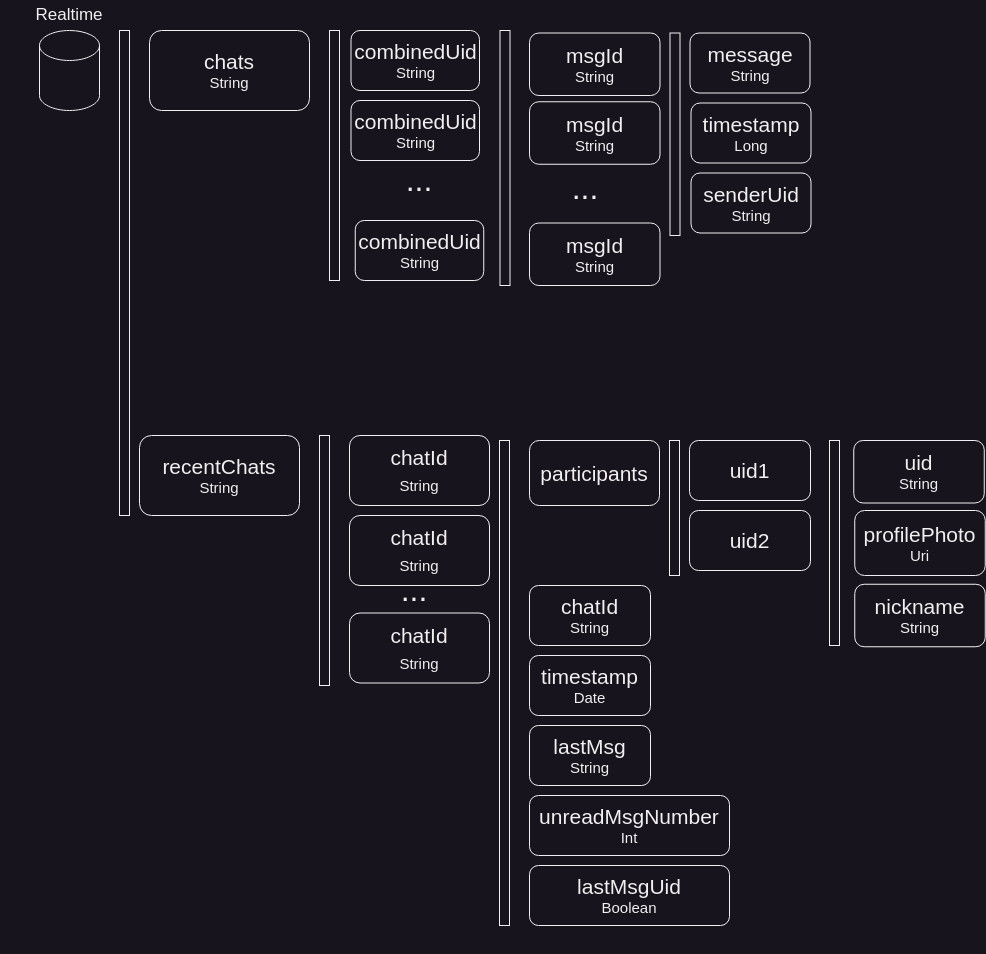
\includegraphics[width = 0.9\textwidth]{Imagenes/drawio/realtime_db.jpg}
	\caption{Diseño de la base de datos Realtime usando Drawio.}
	\label{fig:realtime_db}
\end{figure}

\begin{figure}[ht]
	\centering
	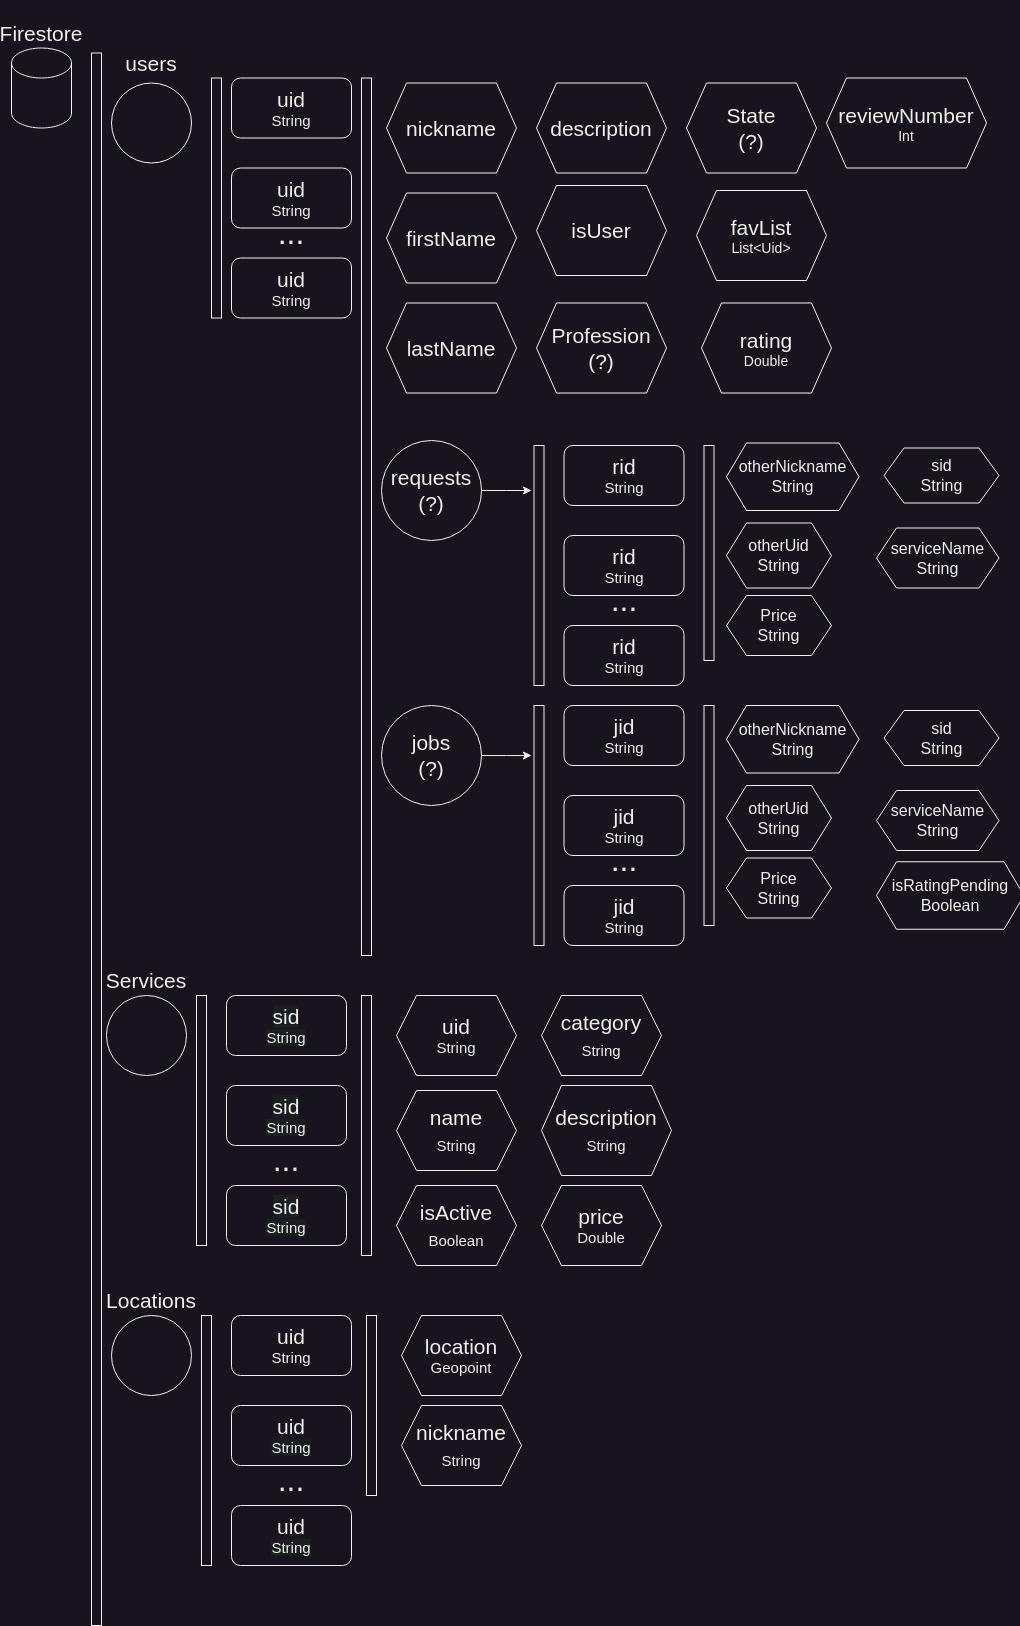
\includegraphics[width = 0.9\textwidth]{Imagenes/drawio/firestore_db.png}
	\caption{Diseño de la base de datos Firestore usando Drawio.}
	\label{fig:firestore_db}
\end{figure}
%\include{...}
%\include{...}
%\include{...}
\backmatter



%
% Índice de palabras
%

% Sólo  la   generamos  si  está   declarada  \generaindice.  Consulta
% TeXiS.sty para más información.

% En realidad, el soporte para la generación de índices de palabras
% en TeXiS no está documentada en el manual, porque no ha sido usada
% "en producción". Por tanto, el fichero que genera el índice
% *no* se incluye aquí (está comentado). Consulta la documentación
% en TeXiS_pream.tex para más información.
\ifx\generaindice\undefined
\else
%%---------------------------------------------------------------------
%
%                        TeXiS_indice.tex
%
%---------------------------------------------------------------------
%
% TeXiS_indice.tex
% Copyright 2009 Marco Antonio Gomez-Martin, Pedro Pablo Gomez-Martin
%
% This file belongs to TeXiS, a LaTeX template for writting
% Thesis and other documents. The complete last TeXiS package can
% be obtained from http://gaia.fdi.ucm.es/projects/texis/
%
% This work may be distributed and/or modified under the
% conditions of the LaTeX Project Public License, either version 1.3
% of this license or (at your option) any later version.
% The latest version of this license is in
%   http://www.latex-project.org/lppl.txt
% and version 1.3 or later is part of all distributions of LaTeX
% version 2005/12/01 or later.
%
% This work has the LPPL maintenance status `maintained'.
% 
% The Current Maintainers of this work are Marco Antonio Gomez-Martin
% and Pedro Pablo Gomez-Martin
%
%---------------------------------------------------------------------
%
% Contiene  los  comandos  para  generar  el índice  de  palabras  del
% documento.
%
%---------------------------------------------------------------------
%
% NOTA IMPORTANTE: el  soporte en TeXiS para el  índice de palabras es
% embrionario, y  de hecho  ni siquiera se  describe en el  manual. Se
% proporciona  una infraestructura  básica (sin  terminar)  para ello,
% pero  no ha  sido usada  "en producción".  De hecho,  a pesar  de la
% existencia de  este fichero, *no* se incluye  en Tesis.tex. Consulta
% la documentación en TeXiS_pream.tex para más información.
%
%---------------------------------------------------------------------


% Si se  va a generar  la tabla de  contenidos (el índice  habitual) y
% también vamos a  generar el índice de palabras  (ambas decisiones se
% toman en  función de  la definición  o no de  un par  de constantes,
% puedes consultar modo.tex para más información), entonces metemos en
% la tabla de contenidos una  entrada para marcar la página donde está
% el índice de palabras.

\ifx\generatoc\undefined
\else
   \addcontentsline{toc}{chapter}{\indexname}
\fi


% Generamos el índice
\printindex

% Variable local para emacs, para  que encuentre el fichero maestro de
% compilación y funcionen mejor algunas teclas rápidas de AucTeX

%%%
%%% Local Variables:
%%% mode: latex
%%% TeX-master: "./tesis.tex"
%%% End:

\fi

%
% Lista de acrónimos
%

% Sólo  lo  generamos  si  está declarada  \generaacronimos.  Consulta
% TeXiS.sty para más información.


\ifx\generaacronimos\undefined
\else
%---------------------------------------------------------------------
%
%                        TeXiS_acron.tex
%
%---------------------------------------------------------------------
%
% TeXiS_acron.tex
% Copyright 2009 Marco Antonio Gomez-Martin, Pedro Pablo Gomez-Martin
%
% This file belongs to TeXiS, a LaTeX template for writting
% Thesis and other documents. The complete last TeXiS package can
% be obtained from http://gaia.fdi.ucm.es/projects/texis/
%
% This work may be distributed and/or modified under the
% conditions of the LaTeX Project Public License, either version 1.3
% of this license or (at your option) any later version.
% The latest version of this license is in
%   http://www.latex-project.org/lppl.txt
% and version 1.3 or later is part of all distributions of LaTeX
% version 2005/12/01 or later.
%
% This work has the LPPL maintenance status `maintained'.
% 
% The Current Maintainers of this work are Marco Antonio Gomez-Martin
% and Pedro Pablo Gomez-Martin
%
%---------------------------------------------------------------------
%
% Contiene  los  comandos  para  generar  el listado de acrónimos
% documento.
%
%---------------------------------------------------------------------
%
% NOTA IMPORTANTE:  para que la  generación de acrónimos  funcione, al
% menos  debe  existir  un  acrónimo   en  el  documento.  Si  no,  la
% compilación  del   fichero  LaTeX  falla  con   un  error  "extraño"
% (indicando  que  quizá  falte  un \item).   Consulta  el  comentario
% referente al paquete glosstex en TeXiS_pream.tex.
%
%---------------------------------------------------------------------


% Redefinimos a español  el título de la lista  de acrónimos (Babel no
% lo hace por nosotros esta vez)

\def\listacronymname{Lista de acrónimos}

% Para el glosario:
% \def\glosarryname{Glosario}

% Si se  va a generar  la tabla de  contenidos (el índice  habitual) y
% también vamos a  generar la lista de acrónimos  (ambas decisiones se
% toman en  función de  la definición  o no de  un par  de constantes,
% puedes consultar config.tex  para más información), entonces metemos
% en la  tabla de contenidos una  entrada para marcar  la página donde
% está el índice de palabras.

\ifx\generatoc\undefined
\else
   \addcontentsline{toc}{chapter}{\listacronymname}
\fi


% Generamos la lista de acrónimos (en realidad el índice asociado a la
% lista "acr" de GlossTeX)

\printglosstex(acr)

% Variable local para emacs, para  que encuentre el fichero maestro de
% compilación y funcionen mejor algunas teclas rápidas de AucTeX

%%%
%%% Local Variables:
%%% mode: latex
%%% TeX-master: "../Tesis.tex"
%%% End:

\fi

%
% Final
%
%---------------------------------------------------------------------
%
%                      fin.tex
%
%---------------------------------------------------------------------
%
% fin.tex
% Copyright 2009 Marco Antonio Gomez-Martin, Pedro Pablo Gomez-Martin
%
% This file belongs to the TeXiS manual, a LaTeX template for writting
% Thesis and other documents. The complete last TeXiS package can
% be obtained from http://gaia.fdi.ucm.es/projects/texis/
%
% Although the TeXiS template itself is distributed under the 
% conditions of the LaTeX Project Public License
% (http://www.latex-project.org/lppl.txt), the manual content
% uses the CC-BY-SA license that stays that you are free:
%
%    - to share & to copy, distribute and transmit the work
%    - to remix and to adapt the work
%
% under the following conditions:
%
%    - Attribution: you must attribute the work in the manner
%      specified by the author or licensor (but not in any way that
%      suggests that they endorse you or your use of the work).
%    - Share Alike: if you alter, transform, or build upon this
%      work, you may distribute the resulting work only under the
%      same, similar or a compatible license.
%
% The complete license is available in
% http://creativecommons.org/licenses/by-sa/3.0/legalcode
%
%---------------------------------------------------------------------
%
% Contiene la última página
%
%---------------------------------------------------------------------


% Ponemos el marcador en el PDF
\ifpdf
   \pdfbookmark{Fin}{fin}
\fi

\thispagestyle{empty}\mbox{}

Este texto se puede encontrar en el fichero Cascaras/fin.tex. Si deseas eliminarlo, basta con comentar la línea correspondiente al final del fichero TFGTeXiS.tex.

\vspace*{4cm}

\small

\hfill \emph{--¿Qué te parece desto, Sancho? -- Dijo Don Quijote --}

\hfill \emph{Bien podrán los encantadores quitarme la ventura,}

\hfill \emph{pero el esfuerzo y el ánimo, será imposible.}

\hfill 

\hfill \emph{Segunda parte del Ingenioso Caballero} 

\hfill \emph{Don Quijote de la Mancha}

\hfill \emph{Miguel de Cervantes}

\vfill%space*{4cm}

\hfill \emph{--Buena está -- dijo Sancho --; fírmela vuestra merced.}

\hfill \emph{--No es menester firmarla -- dijo Don Quijote--,}

\hfill \emph{sino solamente poner mi rúbrica.}

\hfill 

\hfill \emph{Primera parte del Ingenioso Caballero} 

\hfill \emph{Don Quijote de la Mancha}

\hfill \emph{Miguel de Cervantes}


\newpage
\thispagestyle{empty}\mbox{}

\newpage

% Variable local para emacs, para  que encuentre el fichero maestro de
% compilación y funcionen mejor algunas teclas rápidas de AucTeX

%%%
%%% Local Variables:
%%% mode: latex
%%% TeX-master: "../Tesis.tex"
%%% End:

%\end{otherlanguage}
\end{document}
